\chapter[Source-target control of PSBN]{Source-target control of partially specified Boolean networks}
\marginpar{
    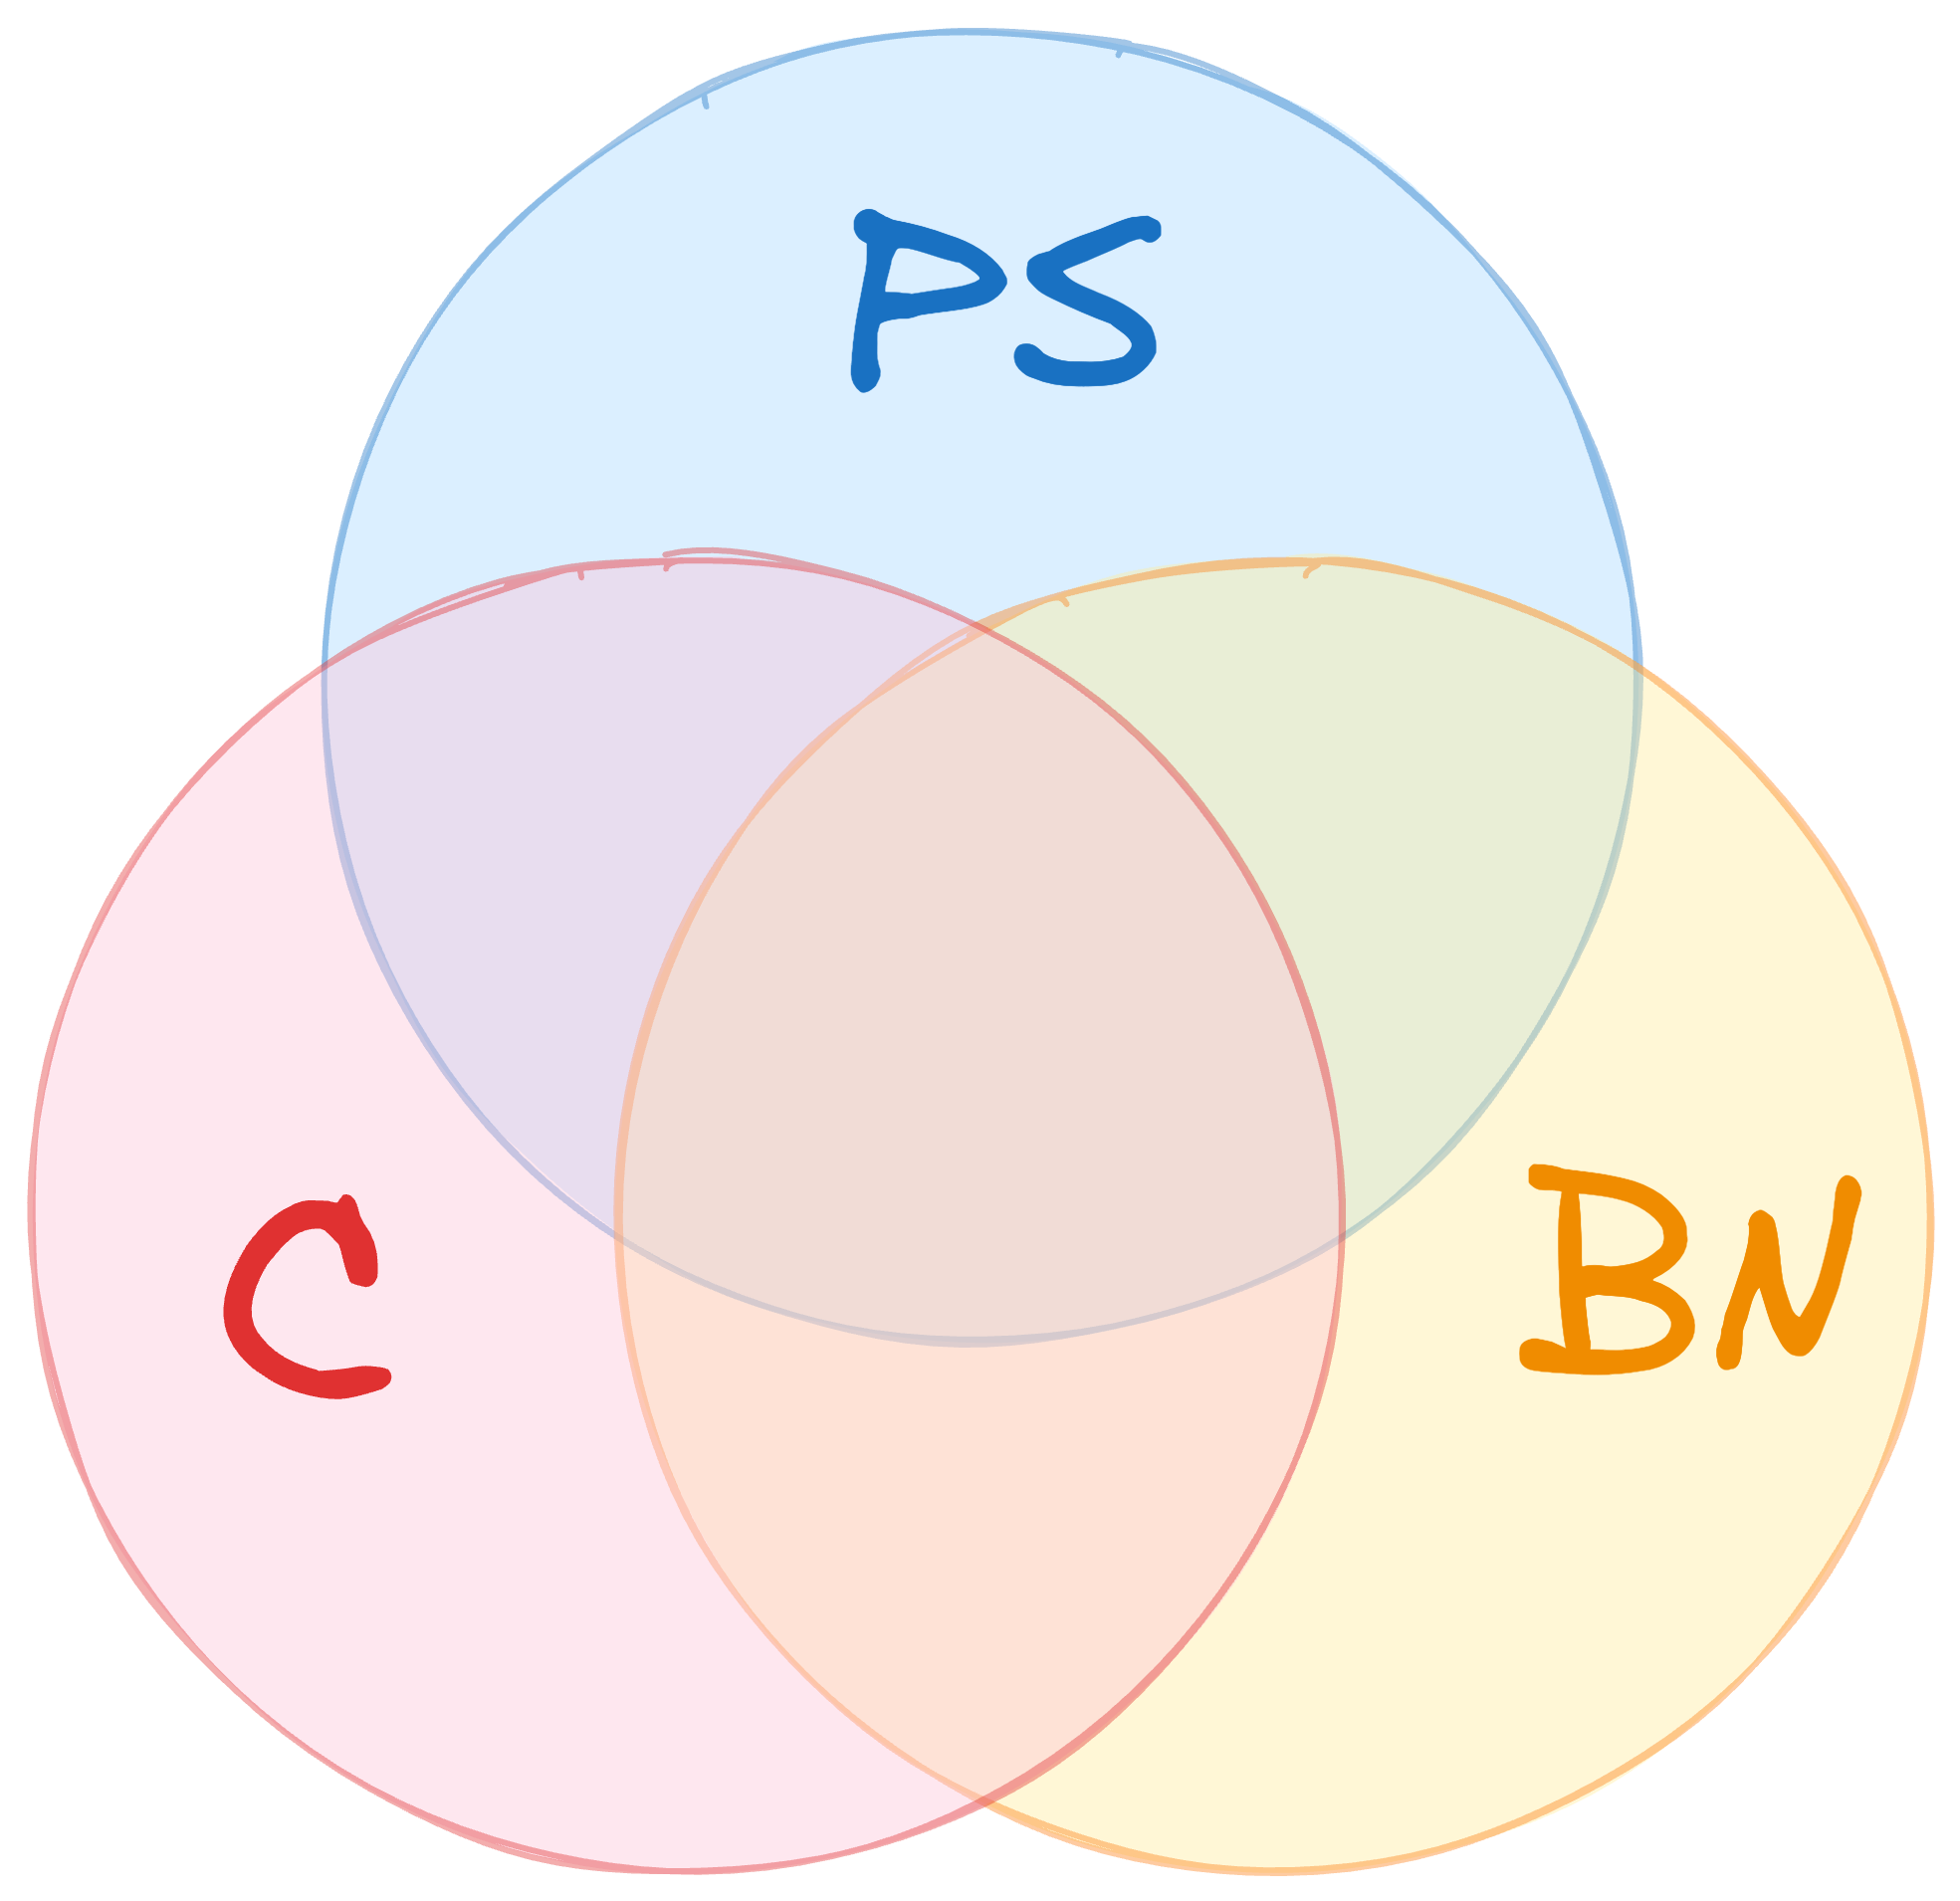
\includegraphics[width=\marginparwidth]{Figures/topics_all.png}
}
\label{chapter:source_target_control}

In our work, the source-target control problem provides a natural starting point for the development of control methods and for understanding the challenges arising from the partial specification of Boolean networks. Since the source state is fixed, it is not necessary to analyze the effect of a perturbation on the entire state space; instead, the search for suitable perturbations can be optimized for the given initial state.

We begin with one-step perturbations, which constitute the simplest class of interventions. As will be shown later, computing one-step perturbations is significantly easier than computing permanent or temporary perturbations, because it does not require modifying the transition system of the network to account for sustained intervention.

However, one-step perturbations are often less efficient than perturbations applied over a longer time horizon. Therefore, we also develop methods for permanent and temporary perturbations, which are computationally more complex but may yield smaller perturbation sets.

In this chapter, we first define the source-target control problem in \autoref{s:source_target_problem_definition}, including the notions of one-step, permanent, and temporary perturbations. Next, in \autoref{sec:target_semisymbolic}, we present a symbolic method for computing one-step source-target control in partially specified Boolean networks. Finally, in \autoref{sec:ostp_symbolic}, we extend this method by representing the state space of perturbed networks so as to handle permanent and temporary perturbations as well.


\section{Problem definition}
\label{s:source_target_problem_definition}

The cardinal difference between classical Boolean networks and partially specified Boolean networks is that the latter can be interpreted in many ways, depending on the chosen parameter valuation. As a consequence, the state transition graph of a PSBN is not uniquely defined. Instead, every interpretation induces a different instance of the PSBN, which in turn induces a different state transition graph.

On the other hand, the definition of a perturbation is independent of the network's parametrization. A perturbation simply fixes the values of certain variables to constants. Therefore, the definition of a perturbation is very similar to the one used in classical Boolean networks. 

What we need to keep in mind, however, is the effect of a perturbation on the network's transition system. In a classical Boolean network, a perturbation can be applied to the whole state space, and it simply removes all states that are not admissible by the perturbation. In a PSBN, however, the effect of a perturbation can differ between different interpretations. This is because the unperturbed variables can still evolve freely. As a result, a perturbation can achieve control for some interpretations, while failing for others.

\subsection{Perturbations}

Here, we build on the definitions of perturbations and their applications from the previous chapter. Most notably, we will leverage the concepts of perturbation (\autoref{def:perturbation}), application of a perturbation to a source state (\autoref{def:perturbation_application}), perturbation application to a state-transition graph (\autoref{def:perturbed_stg}) and a perturbed run of a Boolean network (\autoref{def:perturbed_run}).

Now, let us remind the definitions of a perturbation and its application to a source state, but in the context of a partially specified Boolean network (although the definitions themselves remain very similar, since they are independent of the network's dynamics):

\begin{definition}
\label{def:psbn_perturbation}
Assume having a given \PBN{} $\pbnMath = \{\expr_1, \dots, \expr_n \}$. A \emph{variable perturbation} is then a vector $\perturbation \in \bools_\unspecified^n$. For every $\perturbation_i = \unspecified$, we say that the $i$-th variable is \emph{unperturbed}, whereas for $\perturbation_i = 0$ or $\perturbation_i = 1$, we say that the variable is \emph{perturbed}. The \emph{size} of $\perturbation$ is the number of perturbed variables: $\size(\perturbation) = \; \mid \{ i \mid \perturbation_i \neq \unspecified \} \mid$. The set of all considered perturbations is denoted as $\allPerturbations$ and typically equals to $\bools_\unspecified^n$. 
\end{definition}

\begin{definition}
    \label{def:psbn_perturbation_application}
    Given a \PBN{} $\pbnMath = \{\expr_1, \ldots, \expr_n\}$, \emph{application of a perturbation $\perturbation \in \allPerturbations$ to a source state $s \in \bools^n$} is a \emph{forced} state transition, $\pertApply(s, \perturbation) = s \to s'$ such that: 
    $$\pertApply(s_i) = s'_i = \begin{cases}
        s_i & \text{iff } Q_i = \unspecified \\
        Q_i & \text{iff } Q_i \neq \unspecified
    \end{cases}$$
    where $s'$ is the state reached after applying the perturbation.
\end{definition}

\subsection{Perturbed state transition graph and runs}

To facilitate the discussion of temporary and permanent perturbations, we also need to define the effect of a perturbation on the state transition graph of \PBN{}. Since the dynamics of a \PBN{} depend on the chosen interpretation, we also take it to the context for the definitions of the perturbed \PBN{} state transition as well as a perturbed \PBN{} run:

\begin{definition}
    \label{def:psbn_perturbed_stg}
    Let $\widehat{\pbnMath} = \{ \expr_1, \ldots, \expr_n \}$ be a normalized partially specified Boolean network such that $\widehat{\pbnMath}$ admits $m$ nullary function symbols $\allFunSymbols = \{\funSymbol_1, \ldots, \funSymbol_m \}$. Given an $\widehat{\pbnMath}$, and an interpretation $\interpretation \in \allInterpretations$, \emph{application of a perturbation $\perturbation \in \allPerturbations$ to a \PBN{} instance $\widehat{\pbnMath}(\interpretation)$} with $\STG(\widehat{\pbnMath}(\interpretation)) = (\vertices, \edges)$ results in a \emph{perturbed partially specified Boolean network instance} $\widehat{\pbnMath}(\interpretation)_{\perturbation}$ with \emph{perturbed state transition graph} $\STG_{\perturbation}(\widehat{\pbnMath}(\interpretation)) = (\perturbation, \edges_{\perturbation})$ where vertices are a subspace of the unperturbed state space $\vertices = \bools^n$ given by the perturbation $\perturbation$ and a set of perturbed edges $\edges_{\perturbation} \subseteq \edges$ is given as follows:
    $$
    \edges_{\perturbation} = \{(u, v) \mid (u, v) \in \edges \land u \in \perturbation \land v \in \perturbation\}
    $$
\end{definition}

The perturbed STG of a PSBN is illustrated in \autoref{fig:psbn_perturbed_stg}.

\begin{figure}[htb]
	\centering
	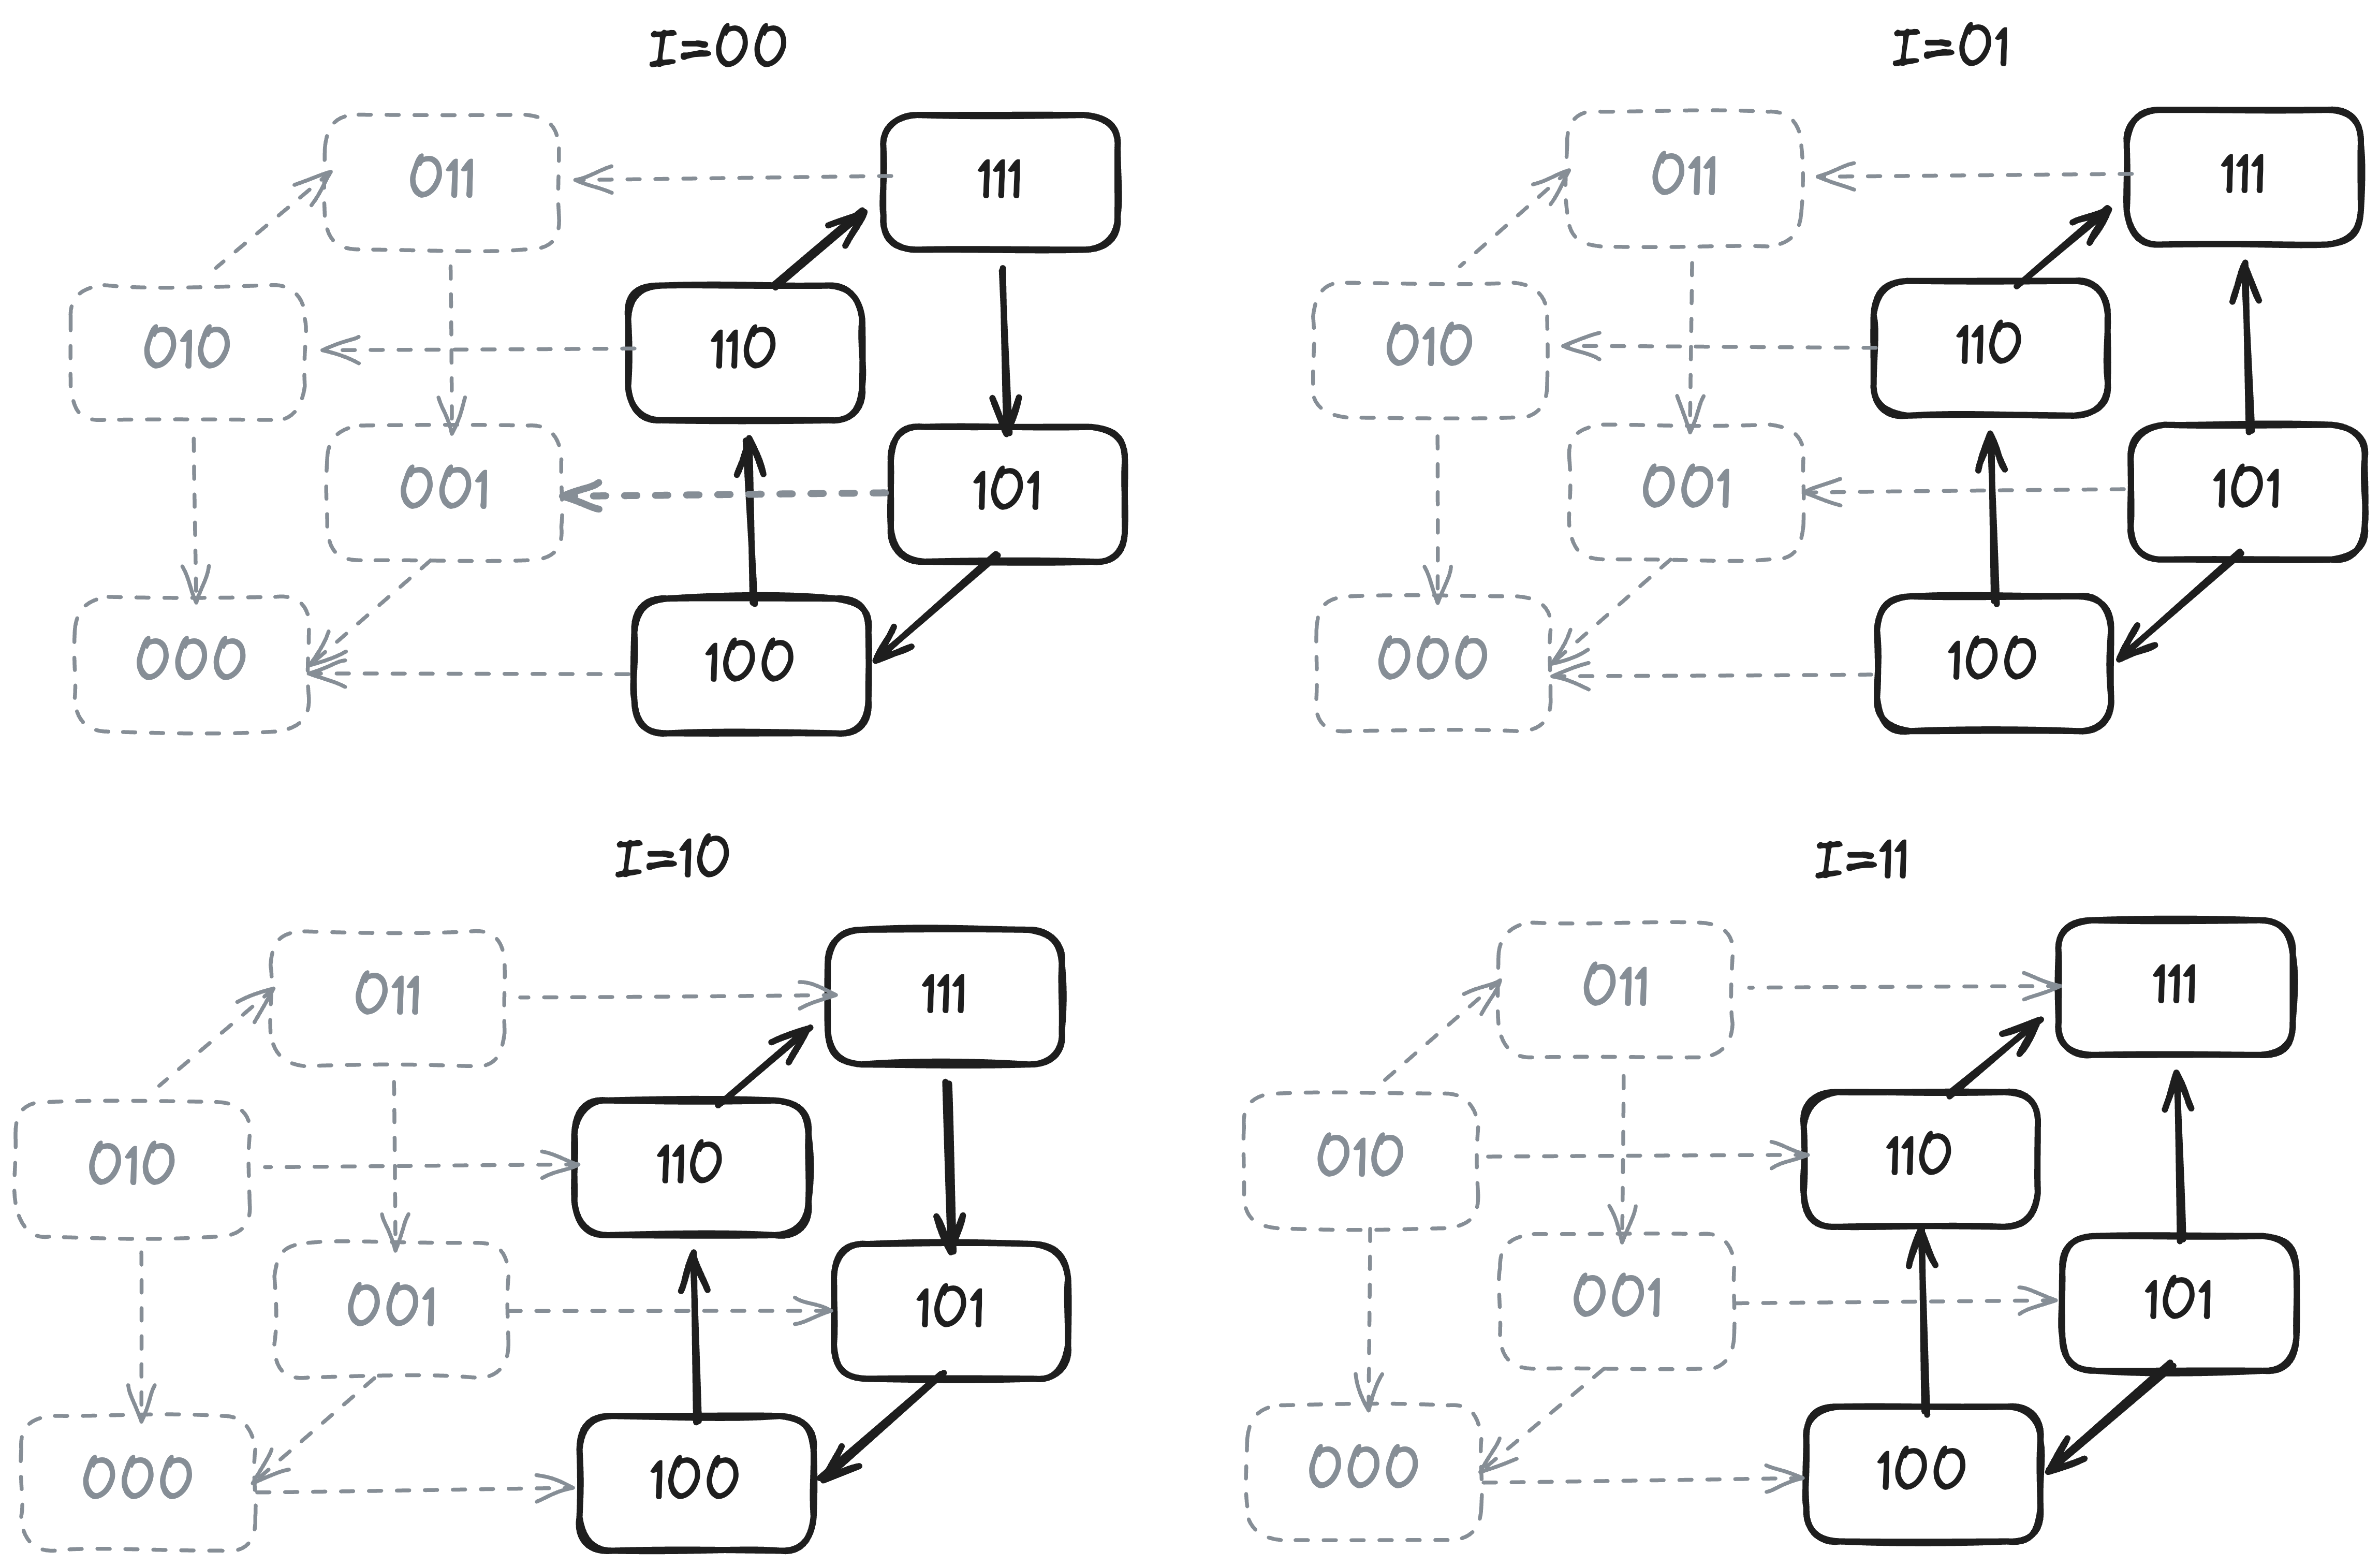
\includegraphics[width=0.8\textwidth]{Figures/psbn_perturbed_stg.png}
	\caption{\textbf{Perturbed STG of a PSBN.} An example of a PSBN with four interpretations perturbed with a perturbation x$1\unspecified\unspecified$.}
	\label{fig:psbn_perturbed_stg}
\end{figure}

\begin{definition}
    Let us assume an interpretation $\interpretation \in \allInterpretations$ of a \PBN{} $\widehat{\pbnMath} = \{\expr_1, \ldots, \expr_n\}$ with $m$ nullary function symbols $\allFunSymbols = \{\funSymbol_1, \ldots, \funSymbol_m \}$ where $\STG(\widehat{\pbnMath}(\interpretation)) = \vertices \times \edges$. Also, have a given source state $s \in \bools^n$, a perturbation $\perturbation \in \allPerturbations$, a and a time period $z \in \Nats_{\infty}$, after which the perturbation is withheld. \emph{A perturbed run $\run_{\perturbation}$} is a run which satisfies the following conditions:
    $$
    \run_{\perturbation}(t) = \begin{cases}
        s & \text{iff } t = 0 \\
        \pertApply(s, \perturbation) & \text{iff } t = 1 \\
        s'  \text{ s. t. } \run(t-1) = s'' \land (s'', s') \in \edges_{\perturbation} & \text{iff }  t'+z > t > t' + 1 \\
        s'  \text{ s. t. } \run(t-1) = s'' \land (s'', s') \in \edges & \text{iff } t > t'+z
    \end{cases}
    $$
    A set $\allRuns_{\perturbation}(\pbnMath(\interpretation), s, z)$ is a collection of all perturbed runs $\run_{\perturbation}$ for a given perturbation $\perturbation$, applied to a state $s$ with perturbation being withheld after $z$ time-steps.
\end{definition}

Notice, that again the definitions of perturbation and its application to a source state remain almost the same as in the \autoref{def:perturbed_run}. The only differences are that we now also consider the interpretation of the \PBN{} instance. Moreover, since this chapter focuses on source-target control, the perturbation is always applied just to a given source state.


\subsection{Control types and goal}
\label{ss:control_types_and_goal}

Finally, we can define the source-target control problem goal in the context of partially specified Boolean networks. Here, we consider three types of perturbations: one-step, permanent, and temporary perturbations. The definitions of these perturbation types are similar to those used in classical Boolean networks~\cite{Su2019CMSB,Su2020}, but adapted to the context of partially specified Boolean networks.

\begin{definition}
\label{def:psbn_control}
Assume having a \PBN{} $\pbnMath = \{\expr_1, \ldots, \expr_n\}$ with $m$ nullary function symbols $\allFunSymbols = \{\funSymbol_1, \ldots, \funSymbol_m \}$, an interpretation $\interpretation \in \allInterpretations$, a source state $s \in \bools^n$, and a target state $t \in \bools^n$ such that $t \in \bigcup \allAttractors(\pbnMath(\interpretation))$. Then, we say that a perturbation $\perturbation \in \allPerturbations$ \emph{controls} $\pbnMath(\interpretation)$ from $s$ to $t$ via:

\begin{itemize}
	\item \emph{One-step perturbation}: if for all $\run \in \allRuns_{\perturbation}(\pbnMath(\interpretation), s, 1)$, $t \in inf(\run)$. That is, after performing the perturbation for a single time-step ($\pertApply(s, \perturbation)$), $t$ is always visited infinitely often without further restricting the network in any way.
	\item \emph{Permanent perturbation}: if for all $\run_{\perturbation} \in \allRuns_{\perturbation}(\pbnMath(\interpretation), \perturbation(s), \infty)$, $t \in inf(\run_{\perturbation})$. That is, $t$ is always visited infinitely often assuming the perturbed variables remain constant to their perturbed value.
	\item \emph{Temporary perturbation}: if for all $\run_{\perturbation} \in \allRuns_{\perturbation}(\pbnMath(\interpretation), \perturbation(s), z+k)$, there exist such time period $z$ that for every $k \in \NatsZero$ we have $t \in inf(\run_{\perturbation})$. Intuitively, the system can evolve for an arbitrary number of time-steps while assuming the perturbed variables are constant. But there must exist some time period $z$ after which if the perturbation is withheld, run reaches (or remains in) $t$ infinitely often.
\end{itemize}

\end{definition}

Here, note several observations regarding the presented types of \PBN{} control. The one-step and permanent perturbations are rather straightforward since they either do not require any further adjustment of the network's transition system (one-step perturbation) or they require a simple restriction of the transition system to the subspace of states admissible by the perturbation (permanent perturbation). The temporary perturbation, however, is more complex since the network transition system needs to be adjusted only for a finite number of time-steps. The number of these time-steps is not know in advance or specific since the Boolean network is not considered to be observable. Typically, we assume, that network reaches some ``intermediate'' attractor within $\edges_{\perturbation}$ an in any of these states, the perturbation can be withheld. Oftentimes, this intermediate attractor contains the target state $t$ itself. In such case, the exact same perturbation works with both temporary and permanent applications.

Moreover, as already noted, the assumption that target state $t$ is a member of an attractor guarantees that if visited once in an unperturbed system, it is in fact visited infinitely often. Second, permanent control could force a particular $t$ to be visited infinitely often even though it is not a member of any attractor in the original $\pbnMath(\interpretation)$. This is because the perturbed variables remain fixed indefinitely, as opposed to one-step and temporary perturbations where the restrictions are eventually lifted. We allow for such case in the phenotype control as we see in the following (\autoref{chapter:phenotype_control_psbn}). Here, to maintain the comparability between all three perturbation types, we strictly restrict ourselves to the interpretations where target is an attractor state.  

Note that under this assumption, any successful permanent perturbation is also successful as a temporary perturbation, since the control can be released once target is reached. If we consider the cases where permanent control can introduce the target attractors, this property no longer holds. Nevertheless, a permanent perturbation can also potentially cause target to not be visited infinitely often by disturbing the attractor in which target resides, or it can cause the attractor to be unreachable within the perturbed state space. In this case, such permanent perturbation simply cannot control the network towards the desired target. An example of such scenario (target being unreachable due to permanent perturbation) is shown in \autoref{ex:only_temporary_working}. 

\begin{figure}
    \centering
    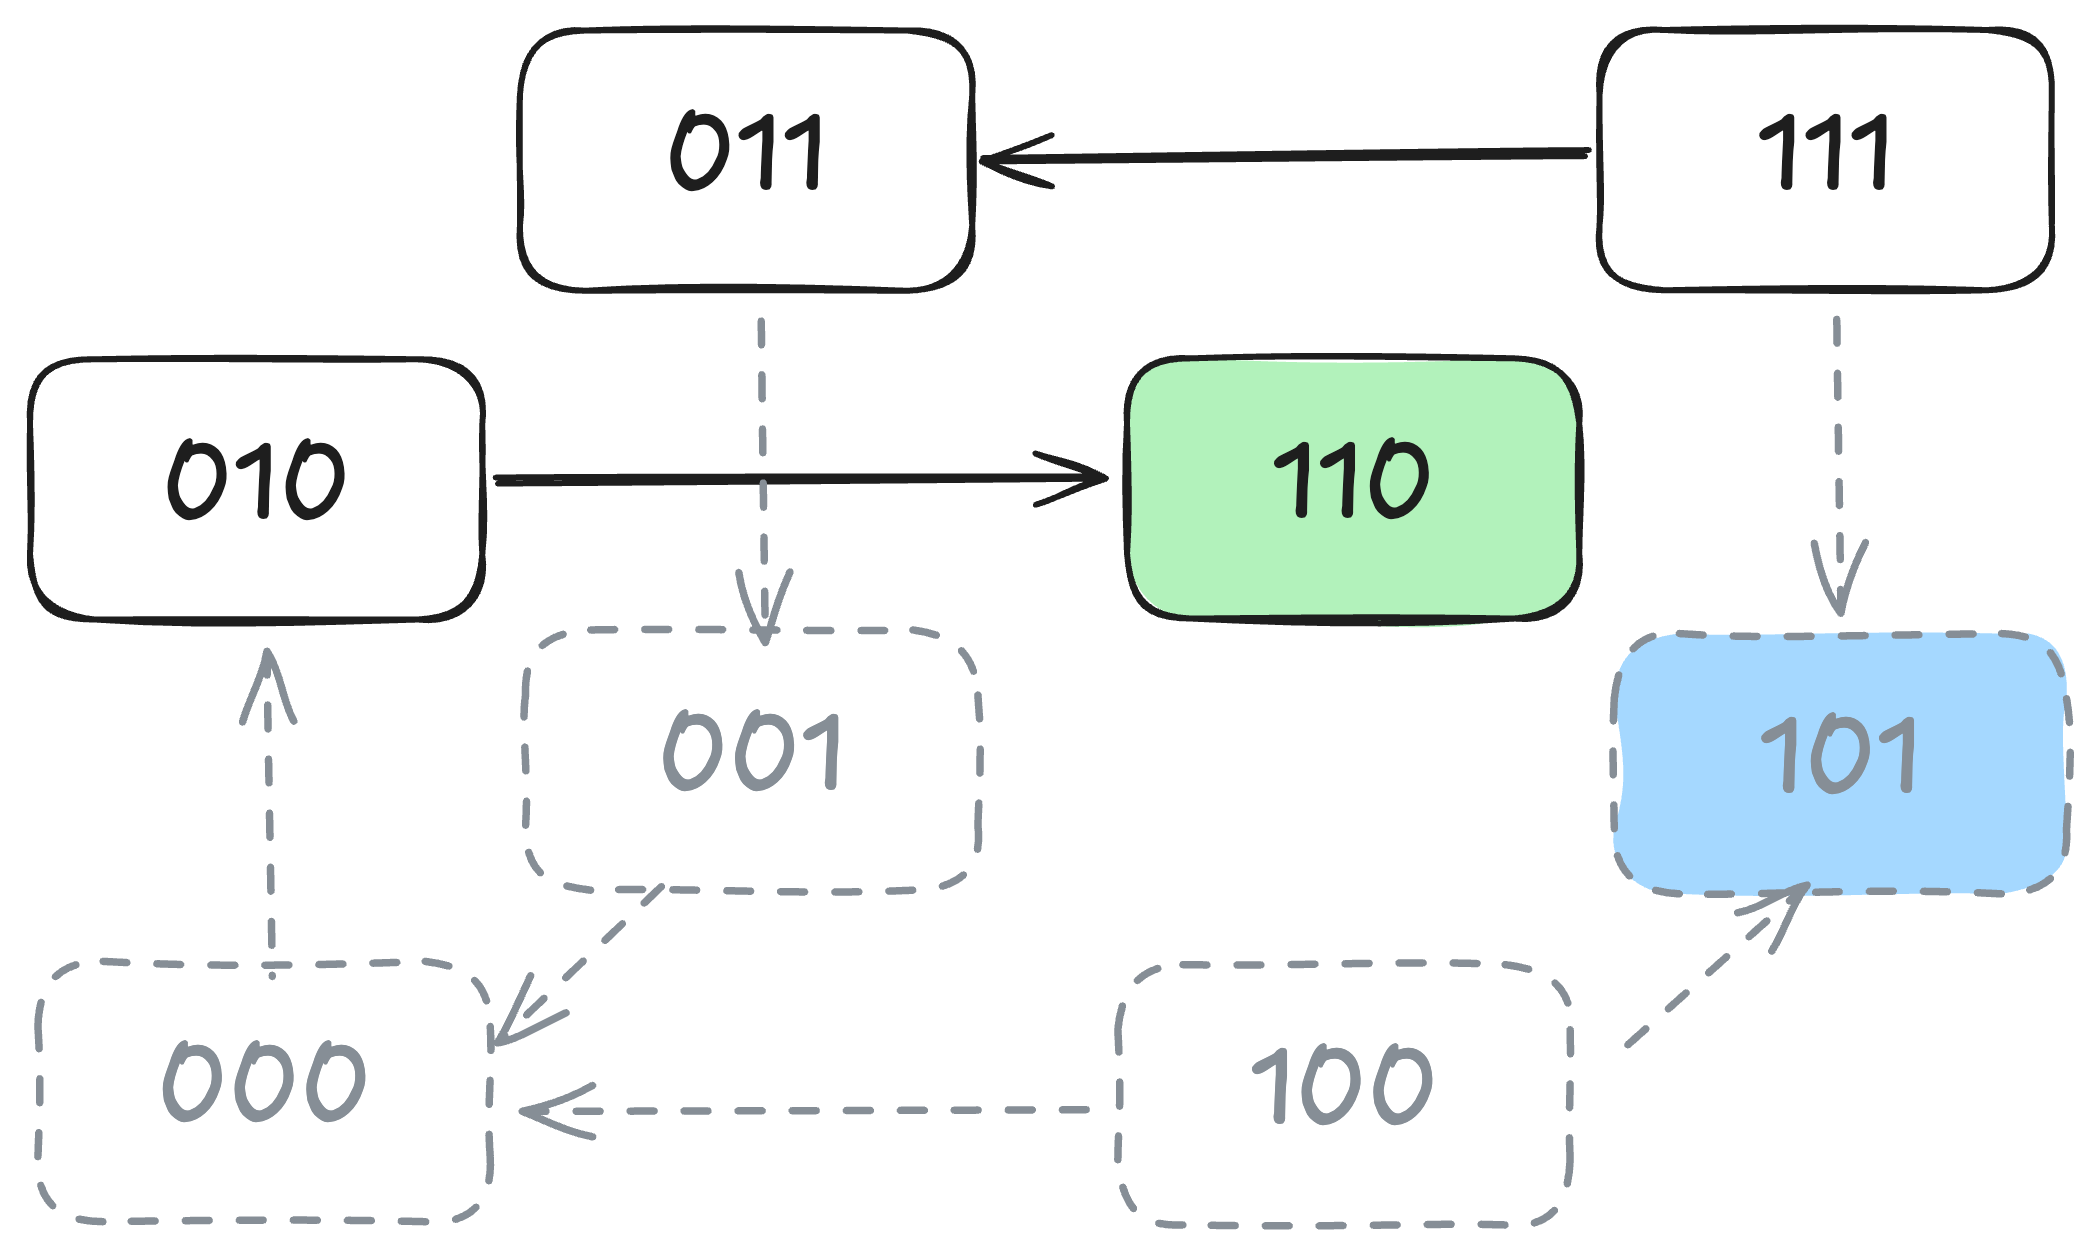
\includegraphics[width=0.45\textwidth]{Figures/only_temporary_working.png}
    \caption{\textbf{A specific case of a perturbed STG.} An example of an STG where a temporary perturbation control the network while one-step or permanent perturbations do not guarantee control.} 
    \label{fig:only_temporary_working}
\end{figure}

\begin{example}
Consider STG from \autoref{fig:only_temporary_working}, source $s = 101$ (blue) and target $t = 110$ (green) with a perturbation $\perturbation = {*}1{*}$. By applying the perturbation, the network transitions from $s=101$ to $\pertApply(s, \perturbation) = 111$. In the shown STG, only solid arrows are admissible while the perturbation is applied. The whole (unperturbed) STG then also admits the dashed arrows. As a result, under permanent perturbation, there is no way of reaching $110$ from $111$. Meanwhile, in the context of a temporary perturbation, $011$ corresponds to a state when the control would be released. Once $011$ is reached, lifting the perturbation guarantees that $target=110$ is eventually reached as well. Finally, note that $\perturbation = {*}1{*}$ is also unsuccessful as a one-step perturbation. This is because by immediately lifting the perturbation, $\pertApply(s, \perturbation) = 111$ can non-deterministically return to $s = 101$---reaching target $t$ is therefore possible, but not guaranteed.
\label{ex:only_temporary_working}
\end{example}

\subsection{Robustness}

In practice, our goal is to not only find perturbations that successfully control the network, but that are efficient and biologically feasible. Indeed, for a target state $t$ any naive perturbation $\perturbation = t$ successfully controls the network towards $t$, but is most likely not realistic. When the network is fully known, we typically focus on finding perturbations that are minimal in terms of size~\cite{Su2019CMSB,Su2020}. This search can be further restricted to network variables where the perturbation is known to be biologically feasible if such information is available.

However, if the network is not fully known, there are many possible interpretations, potentially resulting in very different sets of fair runs. In turn, most perturbations correctly control the network only for some subset of these interpretations. Since we do not know which interpretation (or interpretations) of the PSBN actually occurs in the wild, we may want to quantify such uncertainty. This allows us to search for perturbations that are not only small (in terms of perturbed variables), but that also work for a reasonable portion of the \PBN{} interpretations. Formally, this is captured by the metric of perturbation \emph{robustness}~\cite{Brim2021}:

\begin{definition}
	The \emph{robustness} $\robustness$ of a perturbation $\perturbation \in \bools_\unspecified^n$ for a \PBN{} $\pbnMath$ and a target state $t$ is defined as follows:
	\begin{align*}
		\robustness(\perturbation) = \frac{\mid \{ \interpretation \in \allInterpretations \mid \perturbation~\text{\upshape controls}~\pbnMath(\interpretation) \} \mid}{\mid \{ \interpretation \in \allInterpretations \mid t \in \bigcup \allAttractors(\pbnMath(\interpretation)) \} \mid}
	\end{align*}

	Depending on context, the term \emph{controls} refers to either one-step, permanent, or temporary perturbation as defined above.
\end{definition}

\subsection{Control problem}

As we can see, both size and robustness are critical factors when selecting viable perturbations for a \PBN{}. To facilitate the search for such perturbations and to compare different perturbations, we define control problem for \PBN{} as computation of the \emph{control relation} of all perturbations that successfully control the network from a given source to a given target:

\begin{definition}
\label{def:control_relation}
Given a \PBN{} $\pbnMath = \{\expr_1, \ldots, \expr_n\}$ with $m$ nullary function symbols $\allFunSymbols = \{\funSymbol_1, \ldots, \funSymbol_m \}$, a source state $s \in \bools^n$, and a target state $t \in \bools^n$ such that there exists an interpretation $\interpretation \in \allInterpretations$ for which $t \in \bigcup \allAttractors(\pbnMath(\interpretation))$, the goal of the \emph{source-target control problem} is to compute a \emph{control relation} $\controlRelation_{X}$ -- the set of all pairs $\controlRelation_{X} = \{ \perturbation, \interpretation \} \subseteq \bools_\unspecified^n \times \allInterpretations$ such that $\perturbation$ controls $\pbnMath(\mathcal{I}_c)$ from $s$ to $t$ assuming a type of perturbations $X \in \{ O, P, T \}$ as one-step ($\controlRelation_{O}$), permanent ($\controlRelation_{P}$), or temporary ($\controlRelation_{T}$) control.
\end{definition}

The robustness measure gives us the ability to compare the ``quality'' of a single perturbation. To also compare the ``quality'' of different control relations (or control approaches in general), we extend the notion of robustness to be measurable on a control relation. Specifically, we define \emph{maximal robustness} $\rho_{\max}(\controlRelation_{X})$ to be the maximal robustness achievable by a single perturbation from $\controlRelation_{X}$, and \emph{union robustness} $\rho_{\cup}(\controlRelation_{X})$ to be the collective robustness achievable by all available perturbations: 
\begin{align*}
	\rho_{\max}(\controlRelation_{X}) &= \max_{\perturbation \in \controlRelation_{X}} \rho(\perturbation) \\
	\rho_{\cup}(\controlRelation_{X}) &= \frac{ \mid \bigcup_{\interpretation \in \controlRelation_{X}}\ \interpretation \mid }{\mid \{ \interpretation \in \allInterpretations \mid t \in \bigcup \allAttractors(\pbnMath(\interpretation)) \} \mid}
\end{align*}

Intuitively, the maximal robustness $\rho_{\max}$ gives us the best case scenario that can be achieved using a single perturbation from $Q$. Meanwhile, union robustness $\rho_{\cup}$ is the measure of how well a system can be controlled \emph{overall}. In particular, if union robustness is less than one, there are PSBN interpretations that cannot be controlled by any perturbation in $\allPerturbations$. Both measures are thus worth exploring, as each represents a slightly different optimization goal: While a control relation $\controlRelation_{X}$ with high $\rho_{\max}$ is generally more likely to provide a practically viable control strategy, another control relation with a higher $\rho_{\cup}$ may achieve control even for cases that are not feasible by the former $\controlRelation_{X}$.

\subsection{Summary}

To summarize, in this section we defined the source-target control problem for partially specified Boolean networks. We defined three types of perturbations: one-step, permanent, and temporary perturbations. Then, we defined the goal of the source-target control problem as computation of the control relation containing all perturbations that successfully control the network from a given source to a given target. Finally, we introduced the robustness metric to quantify the uncertainty of a perturbation in terms of the portion of PSBN interpretations it can control.

\section{Semi-symbolic method for one-step control}
\label{sec:target_semisymbolic}

Now we describe our computational framework for solving the one-step state perturbation control of \PBN{}. We start by introducing our approach for finding strong basins in a \PBN{}. Then we explain the framework for exploring \PBN{} STG and for manipulation with \PBN{} interpretations. Next, a concise workflow for \PBN{} control that employs the proposed algorithms is demonstrated. Finally, we present an evaluation of the method on a collection of \PBN{} models. 

\subsection{Semi-symbolic labelled strong basin search}
\label{ss:semi_symbolic_sb}

The foundation of our method is based on binary decision diagram (BDD~\cite{Bryant86}) representation of interpretation sets of a \PBN{}. The decision variables of the BDD are the nullary function symbols of the network meaning that every path from the root to a leaf in such a BDD represent a set of interpretations of the \PBN{} while states are represented explicitly.

Common logical operations on such BDDs (and, or, negation, ...) then correspond to set operations (intersection, union, complement, ...).  Furthermore, static regulation constraints (activation, inhibition, observability) can be formalized using Boolean formulae over interpretations, and we can, therefore, create a BDD which enforces all constraints imposed by the regulatory network and represents the set of only relevant interpretations.

As described in~\autoref{ss:psbn_stg}, \PBN{} dynamics $\STG(\pbnMath{})$ are represented as an edge-labelled state-transition graph, where each transition $s \to t$ has an associated set of interpretations $\interpretationSet(s, t) \subseteq \allInterpretations$ represented as a BDD. A~\emph{labelled state set} is a mapping $\vertices \to 2^{\allInterpretations}$ assigning to each state a set of interpretations. Furthermore, we suppose that the state space is represented \emph{explicitly}, meaning that all operations on states are performed element-wise (typically in parallel).

We consider basic procedures over an STG of a PSBN. Given a source state $s$ and a viable interpretation set $\interpretationSet$ of a PSBN $\pbnMath$, procedures \pre and \post yield a set of labelled states reachable in one step backward/forward from $s$ under interpretations from $\interpretationSet$: 
\begin{align*}
\pre(s, \interpretationSet) = \{ t \mapsto \interpretationSet_t \mid \forall \interpretation \in \interpretationSet_t : \interpretation \in \interpretationSet \land s \to_{\interpretation} t \}\\
\post(s, \interpretationSet) =\{ t \mapsto \interpretationSet_t \mid \forall \interpretation \in \interpretationSet_t : \interpretation \in \interpretationSet \land t \to_{\interpretation} s \}
\end{align*}

These procedures can be then used (e.g. using a fixed-point computation) to compute a maximal labelled state set of \emph{all} forward/backward reachable states from the source state $s$. The set contains all reachable states $t$ where each $t$ is associated with a maximal set of interpretations $\interpretationSet_t$ for which $t$ is reachable from $s$:

\begin{align*}
\fwd(s, \interpretationSet) = \{ t \mapsto \interpretationSet_t \mid \forall \interpretation \in \interpretationSet_t : \interpretation \in \interpretationSet \land s \to^*_{\interpretation} t \}\\
\bwd(s, \interpretationSet) =\{ t \mapsto \interpretationSet_t \mid \forall \interpretation \in \interpretationSet_t : \interpretation \in \interpretationSet \land t \to^*_{\interpretation} s \}
\end{align*}

This representation (explicit state space and symbolic interpretations) allows computing the reachability procedures in parallel. For the underlying implementation, we worked with internal libraries of the tool Aeon~\cite{aeon} which provides most of the necessary functionality, including a convenient format for specifying \PBN{s} and parallel reachability procedures.

For control of \PBN{}, we first need to determine the relevant interpretations $\interpretationSet_A(t)$ for the target state $t$, where $t$ is a part of some attractor. This process is described in \autoref{algo:attractor-params}. The algorithm is following: we first compute all reachable states, but~only the one from which we can also reach back the target state itself are a part of a TSCC. Otherwise, it is possible to reach some other component of the system from the target state, and that contradicts the notion of attractor. In the partially specified setting, we obtain a mapping of states to interpretations in which it is not possible to return to the target again. Therefore, in all these interpretations the target state is not a part of any attractor, and so we discard them from the full parameter space $\allInterpretations$ to obtain $\interpretationSet_A(t)$. 

\begin{algorithm}[h]
	\SetKwInOut{Input}{Input}
	\SetKwInOut{Output}{Output}
	\Input{\PBN{} $\pbnMath{}$, target attractor state $\var{t}$}
	\Output{Attractor interpretations $\interpretationSet_A(\var{t})$}
	\BlankLine
	$\var{F} \gets \fwd(\var{t}, \allInterpretations)$\;
	$\var{B} \gets \bwd(\var{t}, \allInterpretations)$\;
	\tcc{For every state, compute the BDD difference}
	$\var{NA} \gets \var{F} \setminus \var{B}$\;
	\Return{$\allInterpretations \setminus \bigcup_{\var{s} \in \vertices(\pbnMath)}$ \var{NA}(\var{s})}\;
	\caption{Compute attractor interpretations $\interpretationSet_A(\var{t})$.}
	\label{algo:attractor-params}
\end{algorithm}


The key observation for controlling \PBN{s} is that an attractor is always reached from its strong basin (as explained in \autoref{def:basins}). From all other states, it is possible to reach also some other attractor; therefore, reaching the target attractor is not guaranteed. When the attractor's strong basin for all interpretations is known, we can compute the control mapping $\controlRelation_O$ from a source state to the target attractor by considering Hamming differences between the source and the states of the strong basin. 

Our algorithm is based on the fixed-point approach for strong basin computation in fully specified BNs~\cite{Paul2018CMSB}. The premise is that only states from which it is possible to reach the attractor (weak basin) can be part of the strong basin. The weak basin of the attractor is computed using standard reachability algorithms, for example, BFS. Then states are iteratively removed if it is possible to leave the basin from them (and therefore not reach the given attractor). Finally, if there are no states left to remove, the fixed-point is achieved, and the strong basin is found.


\begin{algorithm}[h]
	\SetKwInOut{Input}{Input}
	\SetKwInOut{Output}{Output}
	\Input{PBN $\pbnMath$, target state $\var{t}$, interpretations $\interpretationSet_A(\var{t})$}
	\Output{labelled state set $\vertices \to
		2^{\interpretationSet_A(\var{t})}$ representing the strong basin}
	\BlankLine
	$\var{SB} \leftarrow \bwd(\var{t}, Ap(\var{t}))$\;
	$\var{to\_update} \leftarrow \var{s}$ in $\{ \var{s} \in \vertices \mid \var{SB}(\var{s}) \not= \emptyset \}$\;
	\Do{$\var{to\_update} \neq \emptyset$}{
		$\var{updated} \gets \emptyset$\;
		$\var{to\_remove} \gets \forall \var{s} \in \vertices \rightarrow \emptyset$\;
		\textbf{parallel} \For{$\var{s}$ in $\var{to\_update}$}{  
			\For {$\var{t}$ in $\post(\var{s})$} {
				\tcc{Recompute interpretations leading outside of basin}
				$\var{to\_remove}(\var{s}) \gets \var{SB}(\var{s}) \cap \interpretationSet(\var{s}, \var{t}) \cap (\interpretationSet_A(\var{t}) \setminus \var{SB}(\var{t}))$\;
			}
			\uIf{$\var{to\_remove}(\var{s}) \neq \emptyset$} {
				$\var{updated} \gets \var{updated} \cup \{s\}$ \;
			}
		}
		$\var{to\_update} \gets \emptyset$\;
		\For {$\var{s}$ in $\var{updated}$} {
			\tcc{Update strong basin}
			$\var{SB}(\var{s}) \gets \var{SB}(\var{s}) \setminus \var{to\_remove}(\var{s})$\;
			\tcc{Only predecessors of updated vars might be updated in the next iteration}
			$\var{to\_update} \leftarrow \var{updated} \cup \pre(\var{s})$ \;
		}
	}
	\Return{\var{SB}}\;
	\caption{Parallel strong basin computation.}
	\label{algo:strong-basin}
\end{algorithm} 

In \autoref{algo:strong-basin}, we extend the approach from~\cite{Paul2018CMSB} onto \PBN{}. For each state we remember under which interpretations it is in the basin, starting with the labelled weak basin (backward reachability from the target state). Then we iterate over the basin's states. For~each state, we consider its successors, and we compute the interpretations for which some successor is \emph{not in the strong basin}. In these interpretations, it is possible to leave the basin, and therefore these interpretations are not part of the strong basin and so we remove them for this state. 

We can process the states in parallel and compute for them the interpretations which are not part of the strong basin. To avoid writing to the strong basin structure while it is intensively read from, we store the interpretations which should be removed separately, and after it is computed, we update the strong basin structure sequentially. The procedure is repeated until nothing more can be removed from the strong~basin.

\subsection{Control computation workflow}

Now we can describe a complete workflow for computing the source-target control in \PBN{s}, depicted in \autoref{fig:workflow}. The~workflow consists of three inputs and three computation steps, resulting in the control mapping $\controlRelation_O$. 

Given an input \PBN{} and a target attractor state $t$, we start by computing valid interpretation set $\interpretationSet_A(t)$ using \autoref{algo:attractor-params}. Then, the labelled strong basin is computed from the \PBN{} with target attractor state $t$ and its valid interpretations $\interpretationSet_A(t)$ using \autoref{algo:strong-basin}. After that, from the strong basin and the source state, we obtain the complete control mapping. Notice that we do not need to know the source state for computing the strong basin and that we can re-use the target's strong basin for obtaining control for different~sources.

To compute the control mapping, observe that viable controls correspond exactly to the Hamming differences (the variables with opposite values) between the source state and the states of the strong basin; yielding one viable perturbation $\perturbation$ for every state $s$ in the strong basin $\var{SB}$. Any other control $\perturbation'$ does not reach the strong basin and therefore does not guarantee to reach the target attractor (for these, $\controlRelation_O(\perturbation) = \emptyset$). A perturbation $\perturbation$ is then viable only for interpretations for which $s$ appears in the strong basin, we thus set $\controlRelation_O(\perturbation) = \var{SB}(s)$. 

\begin{figure}
\checkoddpage
\edef\side{\ifoddpage l\else r\fi}
\makebox[\textwidth][\side]{% 
	\begin{minipage}{\fullwidth}
	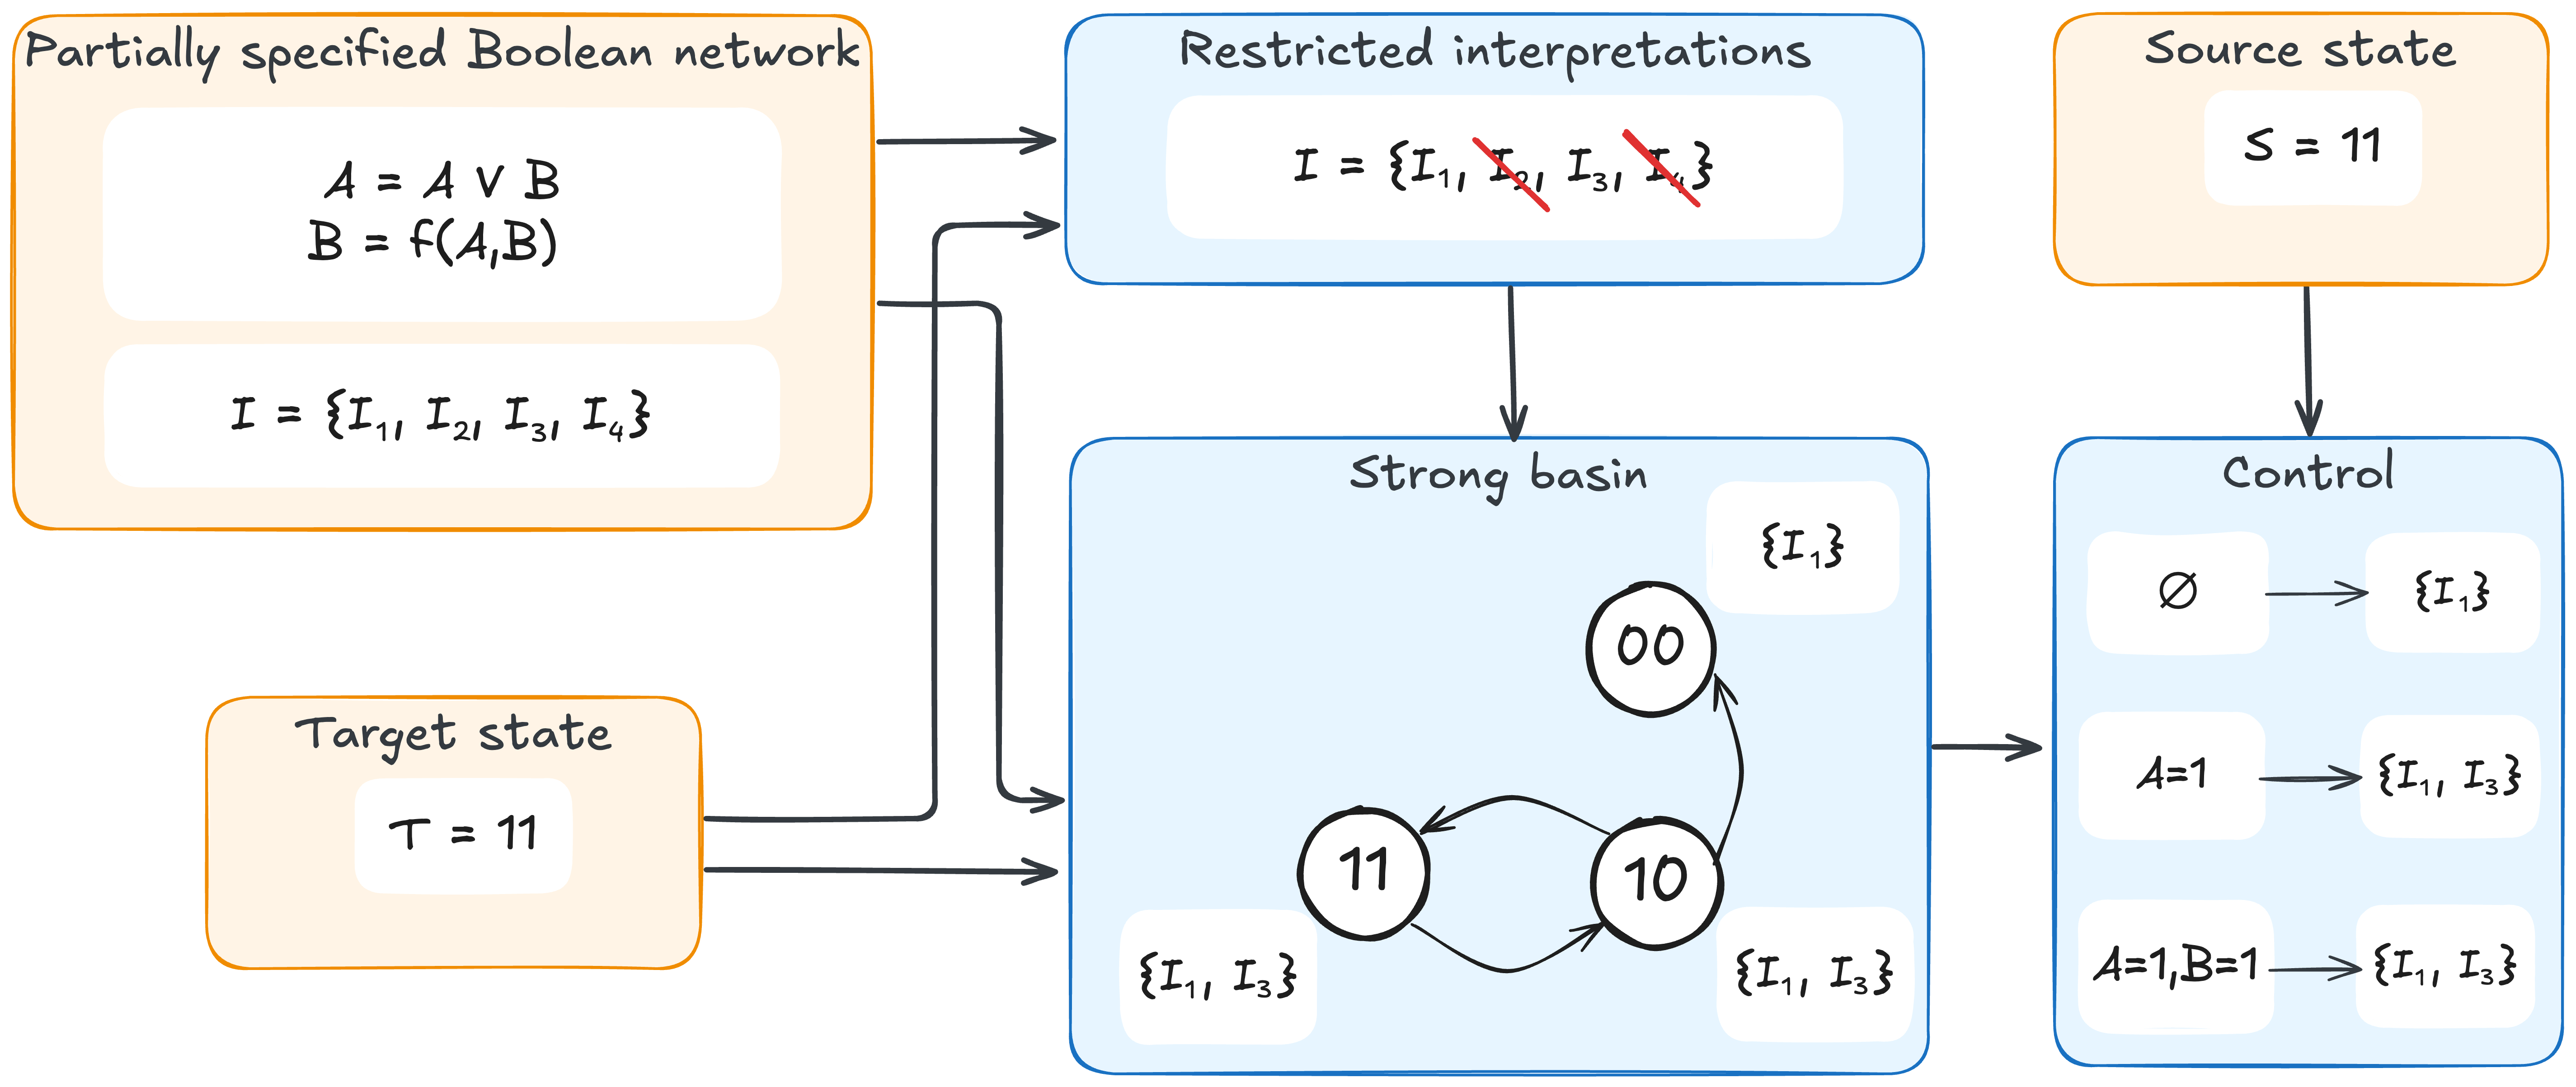
\includegraphics[width=\textwidth]{Figures/workflow.png}
	\caption{
		\textbf{Workflow of computing the source-target control problem.} Parts in the orange boxes represent inputs and blue boxes represent (intermediate) results.
	}
	\label{fig:workflow}
\end{minipage}%
}%
\end{figure}

% Is the 2nd subfigure (Restricted parametrisation Ap) correct?
% Authors: Yes.


Finally, we can compute the size and robustness of each control as we have all knowledge regarding the variables which need to be controlled and interpretations for which the controls work. If it is desired, we can construct a \emph{witness} \PBN{} instance for a perturbation $\perturbation$ (a fully specified BN where the given control works) by fixing the parameters from $\controlRelation_O(\perturbation)$.

In complex and highly unspecified models, it is not unusual for empty perturbation $\emptyset$ to control the network where in some interpretations and therefore no action would be needed to control the model. This is because, in some interpretations, the source might already be a part of the target's strong basin. If this case is considered unrealistic (since there is probably a need for control, thus these interpretations appear to be invalid), the interpretations $\interpretationSet_A(t)$ can be replaced with a custom set of~interpretations.

The resulting set of all available controls can be then used for e.g., cell reprogramming. However, we might obtain many possible controls, and we need to decide which one should be applied. To do that, we can decide based on the size of control or its robustness. The control set can be arbitrarily filtered discarding controls with size bigger than the trivial control (which always has 100\% robustness) or bigger than some set size. Similarly, the control relation can be pruned based on too low robustness. It is left to the actual application to decide which control would best suit its needs. Namely, whether it is more important for the control set to be small or to be robust, as typically, there is rarely available perturbation which would be optimal in both these factors.

% \enlargethispage*{5mm}
\subsection{Results}

\label{sec:results}
We evaluate our approach on two real-life BN models. We compare the performance of our approach using a different number of parameters implanted into the models, resulting in different size of relevant parameter space. We conducted all measurements using a machine equipped with AMD Ryzen Threadripper 2990 WX 32-Core Processor and 64 GB of~memory.

The first model is a \emph{cell-fate decision model}~\cite{Calzone2010}. The model provides a high-level view of possible different cell fates such as pro-survival, necrosis or apoptosis. We used an adapted version of this model, where only regulatory network is provided and all the functions are left unspecified. Then, we selected seven biologically relevant attractors and computed strong basins only for these attractors in several model instances differing in the number of unknown parameters (see \autoref{table:results}).

The second model, a \emph{myeloid differentiation network}~\cite{Krumsiek2011}, was designed to model a bone marrow tissue cell differentiation from common myeloid cell to specialised blood cells (megakaryocytes, erythrocytes, granulocytes, and monocytes). The original network has eleven nodes and six attractors. We derived several partially specified versions of the model by arbitrarily substituting update functions of the model for function symbols. Similarly to the previous case, we used only attractors of the original network when computing strong basins for partially specified versions of the model. 
%For both models, we computed the basins of the mentioned attractors. 
The results are again shown in \autoref{table:results}.

% % %\enlargethispage*{5mm}
% % \begin{specialtable}[H]
% %   \tablesize{\small}
	
% % 	%\setlength{\tabcolsep}{0.3em} % for the horizontal padding
% % 	%\renewcommand{\arraystretch}{1.1}% for the vertical padding
% % 	\setlength{\cellWidtha}{\columnwidth/6-2\tabcolsep-0.0in}
% % \setlength{\cellWidthb}{\columnwidth/6-2\tabcolsep-0.0in}
% % \setlength{\cellWidthc}{\columnwidth/6-2\tabcolsep+0.0in}
% % 	\setlength{\cellWidtha}{\columnwidth/6-2\tabcolsep+0.0in}
% % \setlength{\cellWidthb}{\columnwidth/6-2\tabcolsep+0.0in}
% % \setlength{\cellWidthc}{\columnwidth/6-2\tabcolsep+0.0in}
% % \scalebox{1}[1]{\begin{tabularx}{\columnwidth}{>{\PreserveBackslash\centering}m{\cellWidtha}>{\PreserveBackslash\centering}m{\cellWidthb}>{\PreserveBackslash\centering}m{\cellWidthc}>{\PreserveBackslash\centering}m{\cellWidtha}>{\PreserveBackslash\centering}m{\cellWidthb}>{\PreserveBackslash\centering}m{\cellWidthc}}
\begin{table}
	\footnotesize
	\caption{Results of strong basin computation. The values are stated as ranges because we computed strong basins of all attractors considered in the given models. The second column shows the number of model's parameters. The third column shows count ranges of interpretations which contain the given attractor. The fourth and fifth columns display ranges of the number of states in the weak (resp. strong) basins. The last column contains ranges of times needed to compute strong basins.}
	\label{table:results}
	\setlength{\tabcolsep}{4pt}
	\begin{tabular}{llllll}
		\toprule
		\textbf{Model} &  \boldmath$\mid \allFunSymbols \mid$  & \boldmath$\mid \interpretationSet_A(t) \mid$ & \textbf{\# WB States} & \textbf{\# SB States} & \textbf{Time} \\
		\midrule
		\multirow{3}{*}{Cell-Fate}  & 1 & 1 & 258,000--491,184 & 32--352 & 4.4--9.19 s \\ 
		& 8 & 1--4 & 258,000--491,464 & 21--79 & 4.63--13.42 s \\ 
		& 20 & 7--56 & 258,048--491,520 & 1632--262,144 & 5.82--26.59 s \\ 
		\midrule
		\multirow{4}{*}{Myeloid}   & 1 & 1 & 128--1152 & 64--384 & 8--30 ms \\ 
		& 32 & 63--2052 & 224--1984 & 64--1472 & 14--214 ms \\ 
		& 70 & \num{5.9e4}--\num{1.8e7} & 1512--2048 & 256--2048 & 147--1717 ms \\ 
		& 94 & \num{3.4e6}--\num{3.7e9} & 2008--2048 & 1024--2048 & 0.6--15.38 s \\ 
		\bottomrule
	\end{tabular}
\end{table}
% \end{tabularx}}
% \end{specialtable}

Next, we ``virtually'' compare our approach to a na\"ive approach based on an interpretation enumeration (i.e., computing results for each interpretation separately). In~\cite{Baudin2019}, a strong basin of (fully specified) asynchronous BNs is computed using a block decomposition method with 4 ms needed to finish the computation for the \emph{myeloid model}. Even if the reported hardware was slower than in our case, and we assume that the strong basin computation for one interpretation would last only 1 ms, the fully unspecified myeloid model contains an attractor which is present in \num{3.7e9} interpretations. Therefore, the expected time for computing a strong basin for all interpretations with 32-fold parallelization is more than a day compared to less than 27 s achieved using our semi-symbolic approach.

We evaluate the scalability of our approach on a fully unspecified myeloid model. The results are shown in \autoref{table:scalability}. The computation was restricted to the specified amount of CPUs. The final speed-up achieved on our machine, when using 32 CPUs compared to a non-parallel CPU usage was about 10-fold.

% %\enlargethispage*{5mm}
% \begin{specialtable}[H]
%  \tablesize{\small}
\begin{table}
	\caption{\textbf{Scalability of strong basin computation.} The strong basins are computed on attractors of myeloid model~\cite{Krumsiek2011}.}
	\setlength\tabcolsep{0pt}
	\begin{tabular*}{\linewidth}{@{\extracolsep{\fill}}lcccccc}
		\hline
		\textbf{CPUs} &  $\mathbf{\attractor_1}$  & $\mathbf{\attractor_2}$ & $\mathbf{\attractor_3}$ & $\mathbf{\attractor_4}$ & $\mathbf{\attractor_5}$ & $\mathbf{\attractor_6}$ \\
		\hline
		1 & 6.13 s & 99.31 s & 71.32 s & 130.17 s & 45.84 s & 136.65 s \\
		
		2 & 3.34 s & 54.32 s & 38.87 s & 71.31 s & 24.95 s & 74.29 s \\
		
		4 & 1.86 s & 31.3 s & 21.83 s & 40.31 s & 13.71 s & 42.26 s \\
		
		8 & 1.11 s & 19.34 s & 13.31 s & 24.68 s & 8.4 s & 26.49 s \\
		
		16 & 0.87 s & 14.03 s & 9.32 s & 17.56 s & 5.77 s & 18.86 s \\
		
		32 & 0.6 s & 10.98 s & 6.87 s & 13.22 s & 4.54 s & 15.38 s \\
		\bottomrule
	\end{tabular*}
	\label{table:scalability}
\end{table}

Now let us have a look at an example of how the results might be interpreted and a suitable control selected. Suppose that we want to reprogram an erythrocyte cell (attractor having factors \var{EKLF}=1 and \var{GATA-2}=0) into a monocyte cell (attractor having factors \var{cJun}=1 and \var{EgrNab}=1) of the myeloid model. First, we obtain a strong basin of the monocyte attractor having 1472 states yielding us 1472 possible control sets. We can observe that trivial, i.e., the most robust control strategy (setting variables so that we reach the attractor right after applying the control), has size 8. We can discard all controls with size 8 and larger as they are less optimal in all aspects than the trivial control. In our case, there are 1259 controls with a smaller size than the trivial one. 

Resulting smallest control sets have the size 1. However, the~best robustness among these controls is 46\%. Therefore, it is quite likely that it will not work in practice. If we allow the control to have size 2, we can use the control with 76.8\% robustness. Increasing the size further provides control with the size 3 and the robustness 92\% and so is highly likely to reprogram the cell's phenotype. 

To achieve only slightly more robustness (93.8\%), we may use a control of size 5. In this highly unspecified model, there is no control with 100\% robustness being smaller than the trivial one. It is not a rule of the thumb that with bigger size of control we obtain better robustness, for example, the control with the size 11 (the only one, with all variables, reversed compared to the original one) has the robustness of only 50\%. 

It can be seen that the unknown properties of \PBN{} make selection of one particular ``best`` control complicated. The smallest control has low chance to work in reality and while control of size 3 works has significantly better chance to work, the success of the control is not guaranteed and might be difficult to implement. This is why a careful in vitro experimentation is needed to verify the correctness of the control in reality. Nonetheless, the obtained control set still can help and highly reduce the exponential number of potential transcription factor combinations that could be theoretically tested in vitro.

\subsection{Summary}
In this section, we presented a semi-symbolic method for computing the source-target control of \PBN{} using one-step perturbations. The method is based on a fixed-point computation of the labelled strong basin of the target attractor. We demonstrated that our method is capable of controlling highly unspecified models in seconds, and is considerably faster than the na\"ive interpretation scan approach.
%\enlargethispage*{6mm}
% \textcolor{red}{We introduced the control problem for partially specified Boolean networks and we proposed an algorithm for solving the source-target variant of this problem using one-step perturbations. The core procedure of the algorithm is a fixed-point computation of the labelled strong basin of the given target. The method we proposed is semi-symbolic --- it relies on a unique integration of symbolic (based on BDD representation) and explicit (based on enumerative model checking) formal methods. We demonstrated  that our approach is capable if controlling highly unspecified models in seconds. Owing to the doubly exponential explosion of the number of possible parametrisations, such a result cannot be achieved with the na\"ive interpretation scan approach.}

\section{Symbolic method for one-step, temporary and permanent control}
\label{sec:ostp_symbolic}

In the previous section, we presented a method for computing the source-target control of \PBN{} using one-step perturbations. We have seen, that control size for one-step perturbations could be improved. To address this issue, we can consider more general types of perturbations, such as permanent or temporary perturbations. Moreover, in the meantime, the tool AEON was advanced to support symbolic representation of states as well~\cite{benevs2022bdd}, which allows us to explore the whole perturbation space in parallel. Therefore, we can now propose a fully symbolic method for computing the source-target control of \PBN{} using one-step, temporary, and permanent perturbations.

% Real-world partially specified Boolean networks can have a large number of parameters and variables (and consequently, many admissible perturbations). It is not possible to explore the STGs of such networks explicitly. We propose novel symbolic algorithms to address this issue for the problem of BN control. These algorithms are based on the existing approaches for control of fully specified BNs. However, the addition of function symbols introduces extra complexity which we need to address. 

% On the one hand, identifying a single minimal perturbation that is successful for \emph{some} interpretation of the PSBN is not sufficient, as the robustness of such a perturbation can be very low, making it unlikely to work in practice. On the other hand, requiring that the perturbation is effective for \emph{all} possible interpretations may result in unnecessarily large perturbations. To provide a reasonably reliable method, we need to consider a large set of perturbations. Consequently, for performance reasons, our algorithms cannot test only a single perturbation at a time, but need to explore the whole perturbation space symbolically.

\subsection{Symbolic computation model}

Similarly to the previous method, we employ symbolic representation using binary decision diagrams (BDDs)~\cite{Bryant86}. However, in this case, we extend the use of BDDs to represent not just interpretation space symbolically, but also the sets of states. The main advantage of BDDs is that a logical operation (e.g. a conjunction) can be performed directly on two operand graphs, maintaining the compact representation throughout the whole computation. Due to this correspondence, we do not differentiate between a BDD and the Boolean function that it represents. Furthermore, note that any set or relation $X$ consisting of Boolean vectors (e.g. $X \subseteq \bools^k$) can be represented by a Boolean function that returns $1$ exactly for the members of $X$ and $0$ otherwise. Therefore, any such $X$ can be also represented using a BDD. In particular, this includes subsets of network states ($X \subseteq \bools^n$), subsets of PSBN interpretations ($X \subseteq \bools^m$), and relations of the two ($X \subseteq \bools^n \times \bools^m$). Logical operations on BDDs then correspond to set operations (e.g. $\cap \equiv \land$, $\cup \equiv \lor$, etc.).

Another important aspect is that a perturbation $\perturbation$ is not a Boolean vector, but rather a vector over $\bools_\unspecified$. Fortunately, in our algorithms, we do not need to manipulate whole perturbations. Instead, we only encode which variables in the network are perturbed ($q_i = 0$ or $q_i = 1$) and which are free ($q_i = \unspecified$). For this task, subsets of $\bools^n$ are sufficient. To summarize, we use the following notation:
\begin{itemize}
	\item $\vertices \equiv \bools^n$ encodes network states (vertices of $\STG(\pbnMath)$);
	\item $\allInterpretations \equiv \bools^m$ encodes network interpretations (i.e. the set of all possible function symbols valuations);
	\item $\mathbb{L} \equiv \bools^n$ encodes sets of perturbed variables (without the actual perturbation value).
\end{itemize}

Similar to the previous method, target state $t$ may not be an attractor state in all interpretations of the given PSBN. Consequently, instead of $\allInterpretations$, we again consider a smaller subset of interpretations $\interpretationSet_A \subseteq \allInterpretations$ where $t$ is guaranteed to be a member of some attractor. As this requires no functional changes to the presented algorithms, we generally use the set $\interpretationSet_A$, with the implicit assumption that a smaller $\interpretationSet'$ can be also used when desired.

The reason why we do not have to encode full perturbations is because in our algorithms, we use a relation $X \subseteq \vertices \times \allInterpretations \times \mathbb{L}$ to encode the full state of the system. In such an $X$, we assume that if the network is perturbed, only the states that are compatible with the perturbation are permitted within $X$ (this invariant is maintained throughout the algorithms). Consequently, in a triple $(v, 
\interpretation, l) \in X$ where $l_i$ encodes whether a variable is perturbed, $v_i$ encodes either the state of the network (when $l_i = 0$, i.e. unperturbed) or the constant value of the perturbation (when $l_i = 1$, i.e. perturbed).

We then use $\mathbb{X} = \vertices \times \allInterpretations \times \mathbb{L}$ as a shorthand for this extended set of perturbable states and network interpretations. We also write that a pair $(v, l) \in \vertices \times L$ is \emph{equivalent} to a perturbation $\perturbation \in \bools_\unspecified^n$, $(v, l) \equiv \perturbation$, if $\perturbation_i = \unspecified$ when $l_i = 0$, and $\perturbation_i = v_i$ when $l_i = 1$.
% Therefore, to decode full perturbation from the resulting relation $X \subseteq V \times C \times L$, the pairs of $V \times L$ must be considered. 

\begin{figure}[htp]
	\begin{centering}
		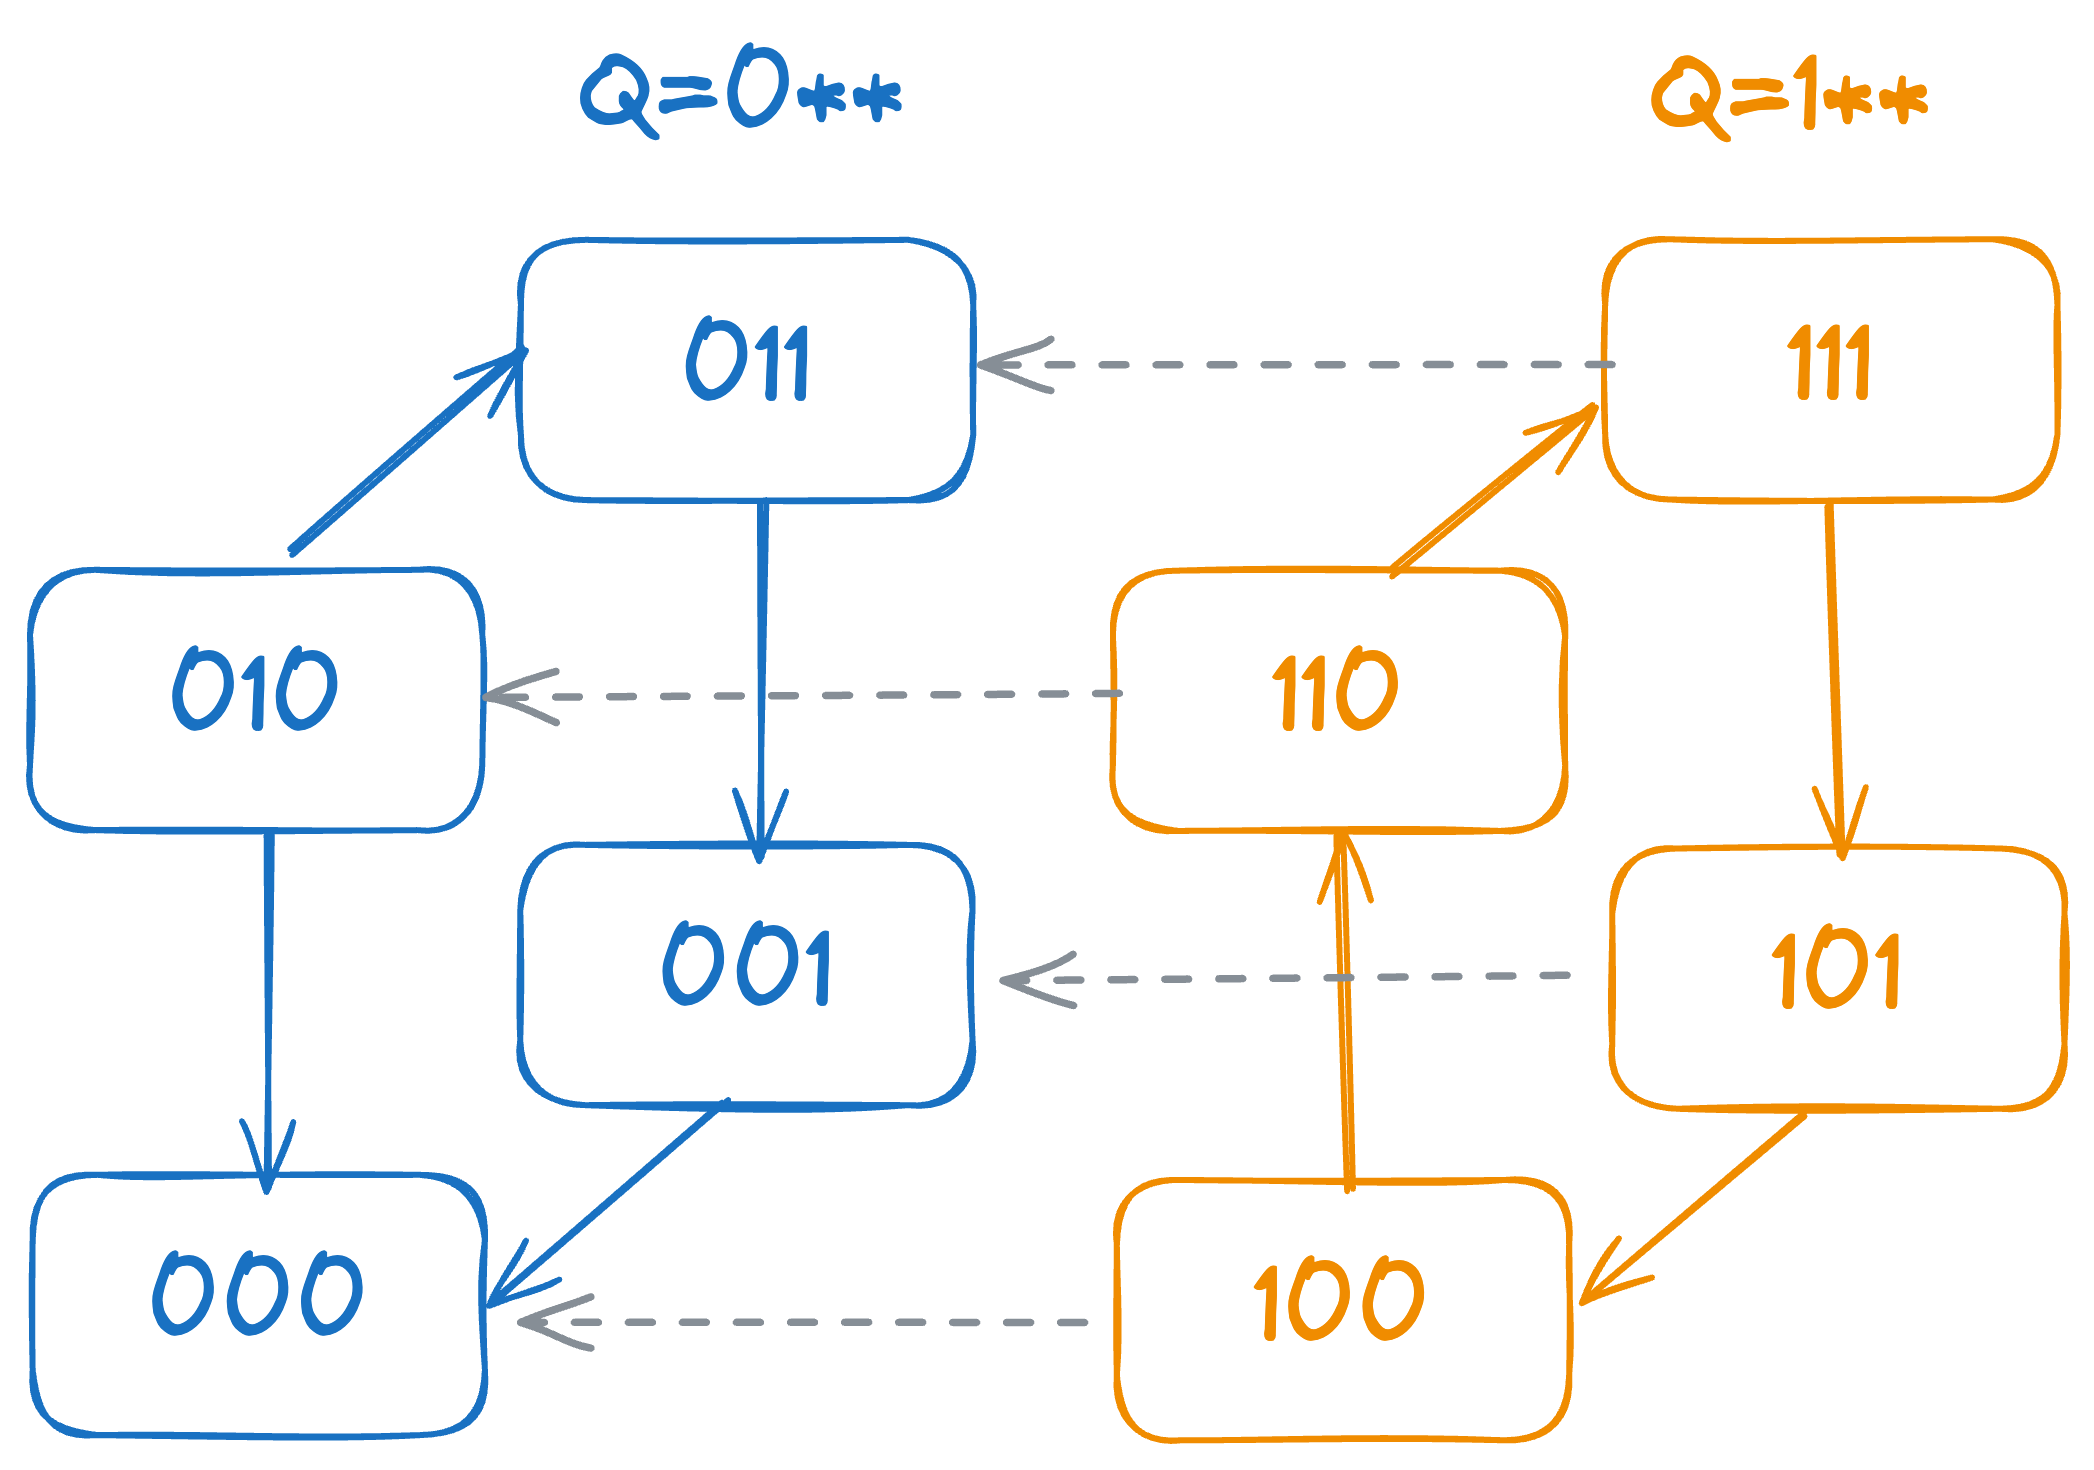
\includegraphics[width=.5\textwidth]{Figures/perturbation_encoding.png}	
		\caption{\textbf{Encoding of perturbations.} Illustration of how perturbations are encoded using pairs of network states and perturbation masks.}
		\label{fig:pert_encoding}
	\end{centering}
\end{figure}

Observe that this approach is more efficient than simply incorporating the set of all possible perturbations $\bools^n_*$ directly into the encoding. Each $\bools_*$ element would require more than one bit per network variable to encode, whereas our approach only adds one bit on top of the existing state space. The details of the decoding for the actual perturbations will be described in \autoref{subsec:supporting_algos}.

\subsection{Symbolic operations}
\label{subsec:symbolic_ops}

Aside from standard set operations ($\cap, \cup, \setminus, \times$, etc.), we also use $\exists_{\mathbb{L}}(X \subseteq \mathbb{X})$ to denote existential projection over the perturbed variables, i.e. $\exists_{\mathbb{L}}(X) = \{ (s, c) \mid \exists l \in \mathbb{L}~(s, c, l) \in X \}$. This can be implemented as a single operation on the directed graph of a BDD as well. Finally, we need a mechanism to symbolically explore the graph $\STG(\pbnMath)$ that is compliant with the applied variable perturbations. For this purpose, we define the following two operations:
\begin{align*}
      \pre(X \subseteq \mathbb{X}) =\; &\{ (s, \interpretation, l) \mid \exists (t, \interpretation, l) \in X \land s \not= t \\ &\land \exists i \in [1,n].t = s[i \mapsto f_i(s) \text{ of } \pbnMath(\interpretation)] \land  l_i = 0 \}\\
      \post(X \subseteq \mathbb{X}) =\; &\{ (t, \interpretation, l) \mid \exists (s, \interpretation, l) \in X \land s \not= t \\ &\land \exists i \in [1,n].t = s[i \mapsto f_i(s) \text{ of } \pbnMath(\interpretation)] \land l_i = 0 \}  
\end{align*}

Recall that the conditions above are almost exactly the condition under which $(v, \interpretation, u) \in E$ of $\STG(\pbnMath)$ (as per \autoref{def:psbn_perturbed_stg}). That is, $\pre$ and $\post$ compute the sets of predecessors and successors of the states in $X$ under their respective $\pbnMath$ interpretations. However, for each computed transition, we also require that $l_i = 0$, i.e. the $i$-th variable is \emph{not} perturbed. Hence values of the perturbed variables remain constant. For example, when $l_i = 1$ for all $i \in [1,n]$, no transition is possible. Meanwhile, when $l_i = 0$ for all $i \in [1,n]$, we get exactly the behaviour of $\STG(\pbnMath)$ without any perturbations. These two operations can also be implemented using BDDs, since $P_i$ is an expression over Boolean variables (which trivially corresponds to a Boolean function and hence a BDD). The rest are either pure logical operations or quantifications that can be realised as BDD operations.

\subsection{Supporting algorithms} 
\label{subsec:supporting_algos}

Our main algorithms rely on a collection of utility procedures defined in \autoref{algo:sb}. Before we proceed with the main result, we quickly explain the rationale behind these procedures. 

\begin{figure}[htp]
	\begin{centering}
		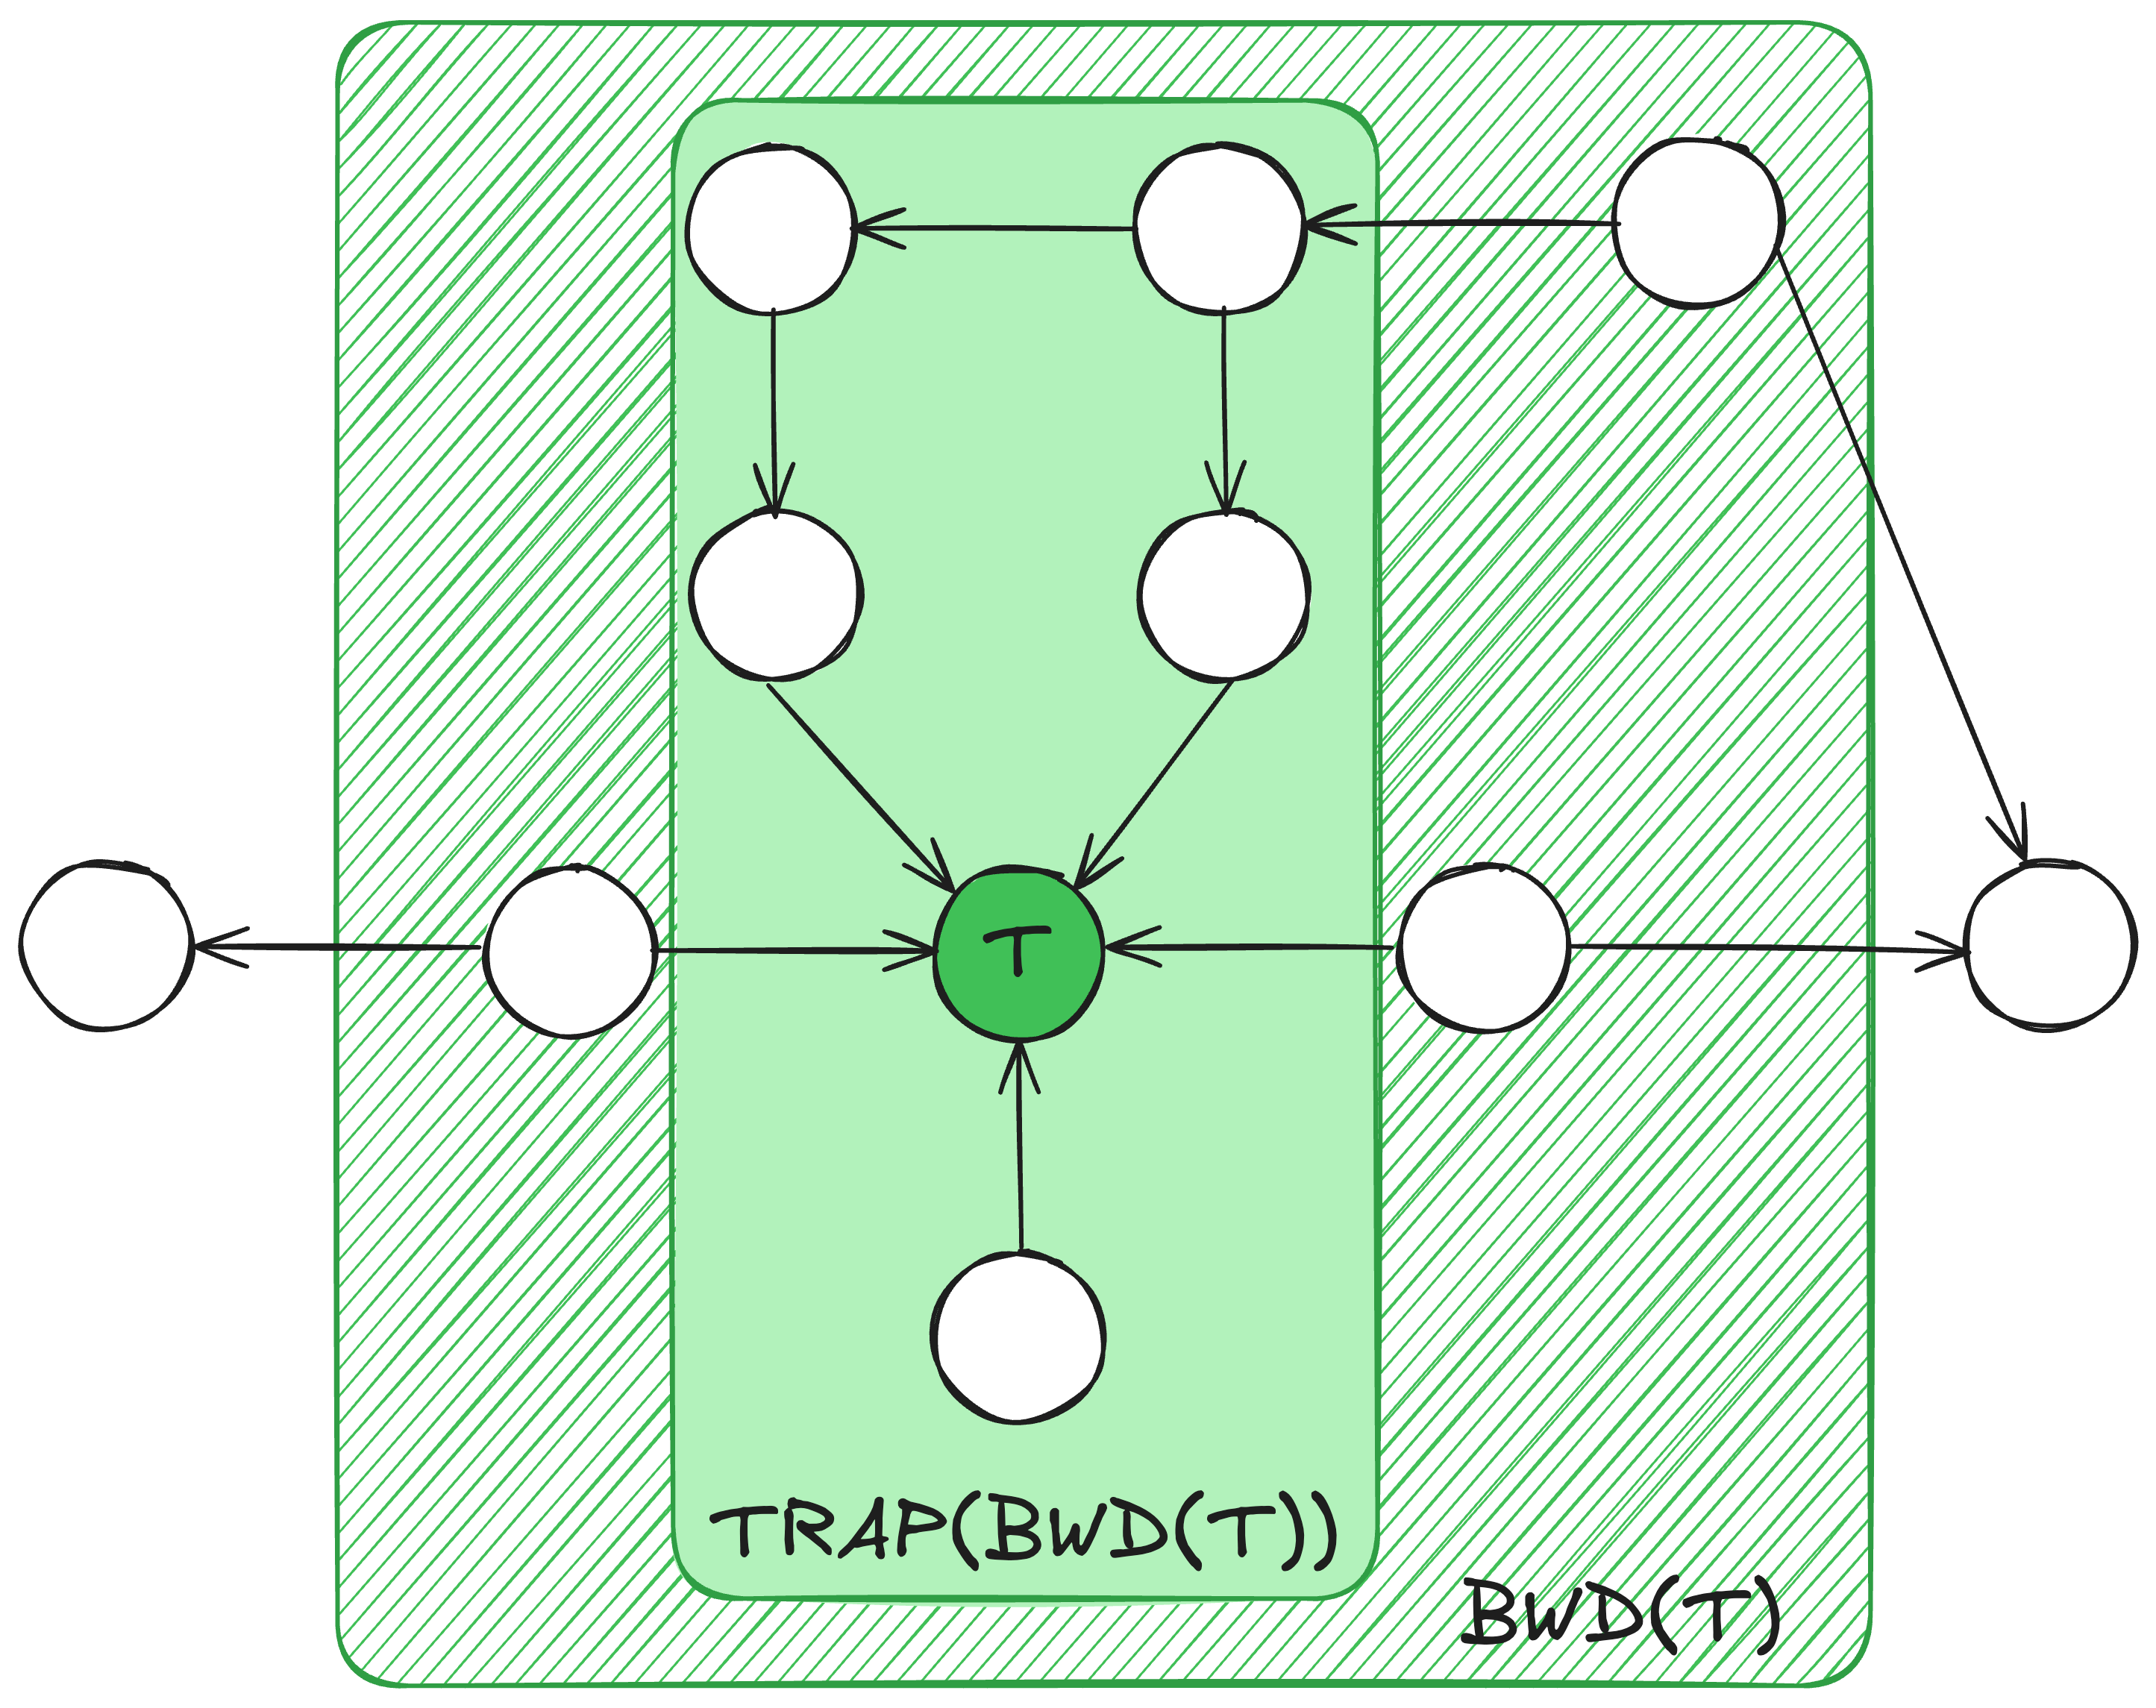
\includegraphics[width=.8\textwidth]{Figures/trap_bwd.png}	
		\caption{\textbf{$\bwd$ and $\fwdClosed$ procedures.} An intuitive example demonstrating the $\bwd$ and $\fwdClosed$ procedures from \autoref{algo:sb}. The highlighted dark green state is the target attractor state $T$. The shaded area represents the set of states $\bwd(\{T\})$ (weak basin of $T$). The solid green area represents the set $\fwdClosed(\bwd(\{T\}))$ (strong basin of $T$).}
		\label{fig:bn_trap_bwd}
	\end{centering}
\end{figure}

\paragraph{\bwd{}} This is a standard backward reachability procedure. That is, for the given set of initial states, it computes all transitive predecessors of these initial states. It also uses our modified notion of state space $\mathbb{X}$ which incorporates information about the perturbed variables. That is, if a variable is perturbed, it cannot be updates (recall our definition of $\textsc{Pre}$).

\paragraph{\fwdClosed{}} This procedure computes a generalized variant of \emph{trap sets} as defined in \autoref{section:boolean-networks}. The procedure takes a set of initial labelled states $X \subseteq \mathbb{X}$ and iteratively eliminates any components that have outgoing transitions leading out of $X$. For unperturbed components, this corresponds exactly to the notion of the trap set (grouped by possible interpretations encoded in the component $C$ of $\mathbb{X}$). For cases where the network is perturbed, the result is still a maximal subset of $X$ with no outgoing transitions, however, only with respect to the unperturbed variables.

\autoref{fig:bn_trap_bwd} shows an example demonstrating the use of $\bwd$ and $\fwdClosed$ (for simplicity, we do not consider multiple network interpretations or perturbations here). Given a target $t$ attractor state, the figure shows the set of all backwards reachable states $\bwd(\{t\})$ (weak basin of $t$). Set $\fwdClosed(\bwd(\{t\}))$ then depicts the maximal trap set contained within $\bwd(\{t\})$ (strong basin of $t$).

\paragraph{\textsc{CanPerturb}} %Finally, the most complex case is the procedure $\textsc{CanPerturb}$. 
Observe that while all procedures introduced so far \emph{respect} existing perturbations (by the means of the $\mathbb{L}$ component of $\mathbb{X}$), no procedure actually \emph{performs} the perturbation step from source $s$ to $\pertApply(s, \perturbation)$ as assumed by all three BN control approaches. However, since our control method works in a bottom up manner, we actually seek to answer a slightly modified question: given a set $T \subseteq \vertices$, what subset $T' \subseteq T$ is reachable from source $s$ by an admissible perturbation? Formally, the goal is to compute triples $(s, \interpretation, l) \in targets$ satisfying $\pertApply(source, \perturbation) = s$ for $\perturbation \equiv (s, l)$ (i.e. $\perturbation$ is the perturbation encoded within the $(s, \interpretation, l)$ triple).

\begin{algorithm}
	\SetKwProg{Fn}{Fn}{}{}
	\Fn{\upshape \bwd$(X \subseteq \mathbb{X})$}{
		\lRepeat{\upshape $X \textbf{ reaches fixpoint}$}{
			$X \gets X \cup \pre(X)$
		}
		\Return{$X$}\;
	} 
	\Fn{\upshape \fwdClosed$(X \subseteq \mathbb{X})$}{
		\tcc{Eliminate elements that escape from $X$ in one step.}
		\lRepeat{\upshape $X \textbf{ reaches fixpoint}$}{
			$X \gets X \setminus \pre(\post(X) \setminus X)$
		}
		\Return{$X$}\;
	}
	\Fn{\upshape \textsc{CanPerturb}$(\var{s} \in \vertices, \var{X} \subseteq \mathbb{X})$}{
		\For{$i \in \{ 1 \ldots n \}$}{
			$\var{diff}_i \gets \{~s' \in V \mid s'_i \not= \var{s}_i~\}$\; 
			$\var{unperturbed}_i \gets \{~l \in \mathbb{L} \mid l_i = 0~\}$\;
			$\var{X'} \gets \var{X} \setminus (\var{diff}_i \times \mathbb{L} \times \var{unperturbed}_i)$\;
		}
		\Return{\upshape $\var{X'}$}\;
	}
	\caption{Basic graph algorithms.}
	\label{algo:sb}x
\end{algorithm}    


To compute $\textsc{CanPerturb}(s, X)$, need we respect the following: Let $(s', \interpretation, l) \in X$ be a triple such that $s'_i \not= s_i$ and $l_i = 0$ for some $i \in [1,n]$. That is, source $s$ and $s'$ differ in the value of the $i$-th variable, but the variable is marked as unperturbed in $l$. Then, and only then we have that $\pertApply(s, \perturbation) \not= s'$ for $\perturbation \equiv (s, l)$. In other words, every $(s, c, l)$ for which such variable exists must be removed from $X$ when computing $\textsc{CanPerturb}$. \autoref{algo:sb} thus iterates through all network variables, constructing a symbolic representation of the set of triplets which violate the aforementioned condition, and subtracting this set from the original $X$. The result is a subset of the $X'$ relation where every member is reachable from source $s$ via its respective perturbation.

\subsection{Control algorithms}
\label{ss:control_algos_st_otp}

In \autoref{algo:permanent},  we describe the bottom-up procedures which compute the relations $\controlRelation_O$, $\controlRelation_P$, and $\controlRelation_T$. Each algorithm relies on the procedures from \autoref{algo:sb}, but incorporates specific adjustments to accommodate the temporal aspects of a specific control approach.

\begin{algorithm}
  \SetKwProg{Fn}{Fn}{}{}
  \Fn{\upshape \textsc{Permanent}$(\var{s} \in \vertices, \var{t} \in \vertices)$}{
    $\var{basin} \gets \fwdClosed(\bwd(\{ \var{t} \} \times \allInterpretations \times \mathbb{L}))$\;
    $\var{map} \gets \textsc{CanPerturb}(\var{s}, \var{basin})$\;
    \Return{\upshape $(\perturbation, \interpretation) \in \controlRelation_{P} \Leftrightarrow (s,\interpretation,l) \in \var{map} \land (s,l) \equiv \perturbation$}\;
  }
  \Fn{\upshape \textsc{OneStep}$(\var{s} \in \vertices, \var{t} \in \vertices)$}{
    $\var{basin} \gets \fwdClosed(\bwd(\{ \var{t} \} \times \allInterpretations \times \{ 0 \}^n))$\;
    $\var{basin} \gets \exists_\mathbb{L}(\var{basin}) \times \mathbb{L}$\;
    $\var{map} \gets \textsc{CanPerturb}(\var{s}, \var{basin})$\;
    \Return{\upshape $(\perturbation, \interpretation) \in \controlRelation_{O} \Leftrightarrow (\var{s},\interpretation,l) \in \var{map} \land (\var{s},l) \equiv \perturbation$}\;
  }
  \Fn{\upshape \textsc{Temporary}$(\var{s} \in \vertices, \var{t} \in \vertices)$}{
    $\var{basin} \gets \fwdClosed(\bwd(\{ \var{t} \} \times \allInterpretations \times \{ 0 \}^n))$\;
    $\var{basin} \gets \exists_\mathbb{L}(\var{basin}) \times \mathbb{L}$\;
    $\var{basin} \gets \fwdClosed(\bwd(\var{basin}))$\;
    $\var{map} \gets \textsc{CanPerturb}(\var{s}, \var{basin})$\;
    \Return{\upshape $(\perturbation, \interpretation) \in \controlRelation_{T} \Leftrightarrow (\var{s},\interpretation,l) \in \var{map} \land (\var{s},l) \equiv \perturbation$}\;
  }
  \caption{Control procedures.}
  \label{algo:permanent}
\end{algorithm}  

\paragraph{\textsc{Permanent}} The procedure for computing permanent control is the most straightforward. First, we use $\bwd(\{t\} \times \allInterpretations \times \mathbb{L})$ to determine all states that are able to reach $t$ across all possible PSBN interpretations ($\allInterpretations$) and combinations of perturbed variables ($\mathbb{L}$). Procedure $\fwdClosed$ then retains only the states from which all runs are guaranteed to eventually reach $t$. This follows from the fact that $t$ is a member of the only attractor within the initial set, hence fair runs that do not leave $\bwd(\{t\} \times \allInterpretations \times \mathbb{L})$ must eventually reach it. Finally, $\textsc{CanPerturb}$ is used to determine which of these cases are actually admissible under the given source $s$ . The result is a $\var{map} \subseteq \mathbb{X}$ which describes the control relation $\controlRelation_P$. As $\controlRelation_P$ is not a Boolean relation, it does not have a direct BDD representation---instead, the return statement describes how members of $\controlRelation_P$ correspond to the members of $map$. Intuitively, $map$ can be seen as a simple Boolean encoding of a non-Boolean relation $\controlRelation_P$. 

\paragraph{\textsc{One-step}} Since one-step control does not assume that perturbation is held over time, component $\mathbb{L}$ in the initial states is substituted for $\{ 0 \}^n$. This is a singleton set that only admits the case where no perturbation is applied. By computing $\fwdClosed(\bwd(\{t\} \times \allInterpretations \times \{0\}^n))$, we then get the combinations of states and interpretations which guarantee that $t$ is eventually reached (and visited infinitely often) in the unperturbed network. This corresponds to the strong basin of $t$.

Once $\var{basin}$ is computed, we cannot simply use $\textsc{CanPerturb}$ to identify possible perturbation candidates, as $basin$ only contains cases where the network is unperturbed. Instead, we use $\exists_{\mathbb{L}}(basin) \times \mathbb{L}$ to eliminate the $\{0\}^n$ component from the relation and substitute it for the full set $\mathbb{L}$. Intuitively, this enables all of the possible perturbations within the $basin$, allowing $\textsc{CanPerturb}$ to correctly select cases that are relevant for the given initial $s$ state.

\paragraph{\textsc{Temporary}} Finally, \textsc{Temporary} is conceptually a combination of both approaches: first, a $basin$ is computed with all perturbations disabled (i.e. $\{0\}^n$). At this point $basin$ represents the collection of possible states where lifting the perturbation guarantees that target $t$ is eventually visited infinitely often. Afterwards, $\{ 0 \}^n$ is exchanged for $\mathbb{L}$, which enables all possible perturbations in these $basin$ states. The combination of \bwd{} and \fwdClosed{} is then repeated, yielding a larger set of states that eventually always reach target $t$ even if the corresponding perturbation is initially applied, but eventually lifted (i.e. applied only temporarily). Finally, \textsc{CanPerturb} again limits this set to perturbations that are compatible with source $s$.

Note that under the assumption that $t$ is a member of an attractor for all $\interpretation \in \allInterpretations$, we have that the result of permanent control is always a subset of results for temporary control. Also note that for permanent control, if a combination of perturbed variables disturbs the attractor in which $t$ resides, the $\fwdClosed$ procedure ensures that such case is eliminated from the $basin$ relation entirely. This is because in this situation, all states (including $t$) can reach states that are not backwards reachable from $t$ and are thus eliminated.

Correctness of the procedures follows from the discussion above. All introduced procedures also surely terminate. The fixed-point procedures (\bwd{} and \fwdClosed{}) necessarily reach the fixed-point, because the superset $\mathbb{X}$ on which they operate is finite, and the resulting set can only grow (or shrink) in each iteration. The procedure \textsc{CanPerturb} is a straightforward for-loop over all BN variables. All control procedures are thus a composition of the described terminating operations or symbolic operations on BDDs.

\subsection{Evaluation}
\label{sec:control_evaluation}

To evaluate our methods, we have implemented algorithms from the previous section by using internal libraries of the tool AEON~\cite{aeon}. Our experiments were run using a computer with AMD Ryzen Threadripper 2990WX 32-Core Processor and 64GB of memory. We describe the software implementation and how to access it in the next chapter. %The repository also includes all auxiliary scripts we used for generating partially specified model versions, running the experiments, and visualizing their results.


\subsubsection{Benchmark model set} We use real-world biological BN models to evaluate our methods. The first model is a \emph{myeloid} differentiation network \cite{Krumsiek2011} which models a bone marrow tissue cell differentiation from common myeloid cells to specialised blood cells (megakaryocytes, erythrocytes, granulocytes and monocytes). The second model depicts heart development done by \emph{cardiac} kernel transcription factors~\cite{Waardenberg2014}. The third model explains regulatory interactions, which may cause \emph{ERBB} kinase over-expression -- a marker of breast cancer~\cite{Sahin2009}. The fourth model focuses on specific conditions which lead to a metastatic \emph{tumour}~\cite{Cohen2015}. The last model, the Mitogen-Activated Protein Kinase (\emph{MAPK}) network, consists of signalling pathways involved in diverse cellular processes, such as cell cycle, survival, apoptosis and differentiation~\cite{Grieco2013}. 

As our methods focus on the ability to handle systems with non-trivial unknown behaviour, we synthetically derive partially specified versions of the models listed above. We distinguish six model groups that differ in the number of interpretations (size of $\mid\allInterpretations\mid$). 

The numbers of interpretations corresponding to the individual groups are $[2^0,2^5], [2^6,2^{10}], \dots, [2^{26},2^{30}]$. For every class, we then generate 20 samples of partially specified networks by randomly removing some fully-specified functions. The arity of removed functions is limited to 5 to prevent intractable parameter explosion. This methodology approximates a uniform distribution of samples across an exponential scale of benchmark model sizes while still covering models with varying numbers and arity of uninterpreted functions. %tazky odsek :(

We then also randomly select the target and source attractor for every sampled model. However, we always verify that the actual number of model interpretations admitting the target attractor belongs to the given range. That is, for a model in class $2^{26}-2^{30}$, we guarantee that the target attractor is actually admissible for at least $2^{26}$ interpretations, even though the total number of all possible interpretations for the model can be higher. That is because we optimize control methods by restricting them to the interpretations where the attractor is present. As discussed in \autoref{ss:control_types_and_goal}, one-step and temporary controls are unable to stabilize a system in a state which is not part of any attractor. Since we want the results to be consistent for all methods and phenotypic variation is not the focus of this work, we pose the same constraint to permanent control.

\subsubsection{Scalability}

\begin{figure}[hbt!]
\checkoddpage
\edef\side{\ifoddpage l\else r\fi}
\makebox[\textwidth][\side]{% 
	\begin{minipage}{\fullwidth}
    \centering
    \subfloat[Myeloid (11 variables)~\cite{Krumsiek2011}]{
        \label{subfig:otp_results_a}
	\adjincludegraphics[trim={{0.75\width} 0 0 0},clip,width=0.33\textwidth]{Figures/myeloid_all.pdf}
    }
    \subfloat[Cardiac (15 variables)~\cite{Waardenberg2014}]{
        \label{subfig:otp_results_b}
	\adjincludegraphics[trim={{0.75\width} 0 0 0},clip,width=0.33\textwidth]{Figures/cardiac_all.pdf}
	}
    \subfloat[ERBB (20 variables)~\cite{Sahin2009}]{
        \label{subfig:otp_results_c}
	\adjincludegraphics[trim={{0.75\width} 0 0 0},clip,width=0.33\textwidth]{Figures/erbb_all.pdf}
	}
	\newline
    \subfloat[Tumour (32 variables)~\cite{Cohen2015}]{
        \label{subfig:otp_results_d}
	\adjincludegraphics[trim={{0.75\width} 0 0 0},clip,width=0.33\textwidth]{Figures/tumour_all.pdf}
	}
    \subfloat[MAPK (53 variables)~\cite{Grieco2013}]{
        \label{subfig:otp_results_e}
	\adjincludegraphics[trim={{0.75\width} 0 0 0},clip,width=0.33\textwidth]{Figures/mapk_all.pdf}
	}
    \caption{\textbf{Performance of the control methods.} Plots in every row show results for a different real-world model. The horizontal axis of all plots is showing the number of attractor colors (given by model instances from our benchmark set) and the vertical axis is for the duration (in ms) of the given method computation. Plots in the first three columns show all measurements for one-step, permanent and temporary controls using the colored markers which are surrounded by polygons to better visualize their disposition. The computations that did not finish computation within a threshold of 24 hours are not displayed in the figure. The last column displays scalability trends of all method results by interpolating logistic regression slope with $\log y = \log x$ function.} 
    \label{fig:otp_results}
	\end{minipage}
	}
\end{figure}

Our first experiment evaluates the performance and scalability of our method with respect to the model size (count of variables) and unknown knowledge (number of interpretations). We use the benchmark model set as described above. We list all results in \autoref{fig:otp_results}. All plots are showing the relation of method computation time to the number of considered attractor colors. The rows depict results for particular real-world models. In every column, there are results for different control methods (one-step, permanent, and temporary). The last column displays results from all methods in a single plot. To capture the scalability trends we use $\log y = \log x$ type of logistic regression (due to exponential scaling of colors as well as time). All computations had 24-hour time-out. Nonetheless, this case never occurred for one-step control and only in a MAPK model for permanent control (5 times). The temporary control yields more such cases, but only in the most demanding scenarios in ERBB (2 times), tumour (1 time) and MAPK (70 times) models. Note that as we disregard these results for compact logistic regression visualisation, the logistic regression might be slightly steeper in the reality.

% Our first experiment measures the performance of methods on five biological models with varying state space size (induced by the number of variables), number of interpretations, and possible number of perturbations. All these three components influence the size of the labelled graph under consideration. Whereas the number of vertices is equal to the number of states, the number of all STG instances is equivalent to the product of interpretations and possible perturbations. 

As described before, the symbolic representation is used to encode three types of entities: a set of the STG vertices, a set of interpretations (PSBN interpretations) which admit an edge in the STG, and a set of perturbations that permit the given edge. Therefore, when we increase the number of interpretations, only one dimension of the resulting symbolic representation grows. In opposition, when we increase the number of the system's variables, both the number of states and the number of available perturbations grow. Therefore, it is expected that increasing the model size has a bigger impact on the performance than increasing the number of model interpretations. This hypothesis is to some extent supported by our experiment captured in \autoref{fig:otp_results}. While the maximal increase of variables (myeloid vs. MAPK models) is just five-fold, we need to increase interpretations $10^7$ times to obtain the similar one-step control runtime of the myeloid model as the best-performing MAPK version. This difference is even amplified for other types of control. For example, in the case of temporary control, no myeloid model version performs as bad as the best-performing MAPK. 

Nonetheless, it must be highlighted that the impact of scaling up colours as well as variables is to some extent unpredictable. This is given by the intrinsic mechanics of the introduced STGs. As the nature of our method relies on fixed-point computation where each iteration eliminates only the direct predecessors of a particular set, in cases where e.g. a long path in the graph arises, our method will not be able to scale well: the algorithm will need many iterations to converge, each eliminating only a small fraction of the STG vertices. Another unforeseeable effect on the method's performance have the BDDs themselves. The ordering of the BDD diagram has a significant impact on the effectiveness of all operations and no single ordering strategy can perform best in all cases~\cite{Harlow2001}. Our observation is also supported by the experiment. 

Notice, the high variance of run times for the similar size of attractor interpretations shown in the plots. For example, in the case of temporary control in the ERBB model, compared to versions with fewest interpretations, some highest attractor interpretations (over $10^8$) cause just approximately $10$-times longer execution time while other cases with a similar number of interpretations result in time-outing computations, therefore the slow-down of over $10^7$. Or in the case of the myeloid model, even despite its somewhat smaller variable count than in the cardiac model, some computations take longer than in the bigger cardiac model, especially in the temporary control case. 

Another insight that can be obtained from \autoref{fig:otp_results} is how one-step, temporary and permanent controls differ in their complexity in terms of computational time. We can notice that one-step control is always over-performing other methods. This is because we do not need to consider perturbed state space when computing the trap set of the target attractor. In contrast, temporary control is usually by far the most computationally demanding compared to the other types of control. This should be given by the need to compute two trap sets. The first computed trap set is the same as in the case of one-step control and should be thus easy to compute. 

However, the seed for the second computed trap space is a much bigger vertex set, and therefore the resulting second trap space (which incorporates perturbations) of the first trap space (without perturbations) can generate much more complex symbolic structure and also gives more space for slowly converging fixed-points which were discussed previously. Nonetheless, in some rare cases with models containing few interpretations (myeloid and ERBB), the temporary control might over-perform the permanent one. This can be caused by the first (unperturbed) strong basin computed by temporary control being very similar to the second (perturbed one) while the first computation might be somewhat faster as it does not consider perturbations. We do not observe such scenarios in bigger models (tumor and MAPK)where the trends of one-step over-performing permanent control, and permanent over-performing temporary one look quite consistent.

\subsubsection{Robustness} 

Next, we conduct experiments evaluating the presented robustness metrics across different types of controls. In particular, we use maximal robustness $\rho_{max}$ and union robustness $\rho_{union}$ metrics which we measure on sets of fixed perturbation size. The results are shown in \autoref{fig:maximal_robustness} and \autoref{fig:total_robustness}. 

%For demonstration purposes, we selected just one arbitrary partially specified model instance for every real-world biological network from our benchmark model set, as the perturbation robustness across different randomized models is not directly comparable. 

\begin{figure}[htb!]
\checkoddpage
\edef\side{\ifoddpage l\else r\fi}
\makebox[\textwidth][\side]{% 
	\begin{minipage}{\fullwidth}
	\centering
	\begin{tikzpicture}[scale=0.6, transform shape]
	\begin{axis}[\axisStyle{a) Cardiac (15 variables)}{Maximal}]
		\addplot coordinates {(1,0.095)(2,0.393)(3,0.404)(4,0.599)(5,0.696)};
		\addplot coordinates {(1,0.095)(2,0.685)(3,0.841)(4,0.987)(5,1.0)};
		\addplot coordinates {(1,0.095)(2,0.685)(3,0.841)(4,0.987)(5,1.0)};
		\legend{One-step,Permanent,Temporary}
	\end{axis}
	\end{tikzpicture}
	\begin{tikzpicture}[scale=0.6, transform shape]
	\begin{axis}[\axisStyle{b) ERBB (20 variables)}{Maximal}]
	\addplot coordinates {(1,0.034)(2,0.035)(3,0.036)(4,0.215)(5,0.240)};
	\addplot coordinates{(1,0.215)(2,0.621)(3,0.862)(4,1.0)(5,1.0)};
	\addplot coordinates{(1,0.215)(2,0.621)(3,0.862)(4,1.0)(5,1.0)};
	\legend{One-step,Permanent,Temporary}
	\end{axis}
	\end{tikzpicture}
	\begin{tikzpicture}[scale=0.6, transform shape]
	\begin{axis}[\axisStyle{c) Tumour (32 variables)}{Maximal}]
	\addplot coordinates {(1,0.169)(2,0.197)(3,0.209)(4,0.483)(5,0.563)};
	\addplot coordinates{(1,0.434)(2,0.652)(3,0.869)(4,1.0)(5,1.0)};
	\addplot coordinates{(1,0.434)(2,0.652)(3,0.869)(4,1.0)(5,1.0)};
	\legend{One-step,Permanent,Temporary}
	\end{axis}
	\end{tikzpicture}
	\caption{Maximal robustness $\rho_{max}$ per set of perturbations with a given size -- comparison between different types of controls. The horizontal axis shows the size of perturbations in the set and the vertical axis displays the maximal robustness. Each chart is showing robustness for a different model.}
	\label{fig:maximal_robustness}
	\end{minipage}
}
\end{figure}

\begin{figure}[htb!]
\checkoddpage
\edef\side{\ifoddpage l\else r\fi}
\makebox[\textwidth][\side]{% 
	\begin{minipage}{\fullwidth}
	\centering
	\begin{tikzpicture}[scale=0.6, transform shape]
	\begin{axis}[\axisStyle{a) Cardiac (15 variables)}{Union}]
	\addplot coordinates {(1,0.095)(2,0.395)(3,0.414)(4,0.649)(5,0.743)};
	\addplot coordinates {(1,0.095)(2,0.674)(3,0.962)(4,0.999)(5,1.0)};
	\addplot coordinates {(1,0.095)(2,0.792)(3,0.986)(4,0.999)(5,1.0)};
	\legend{One-step,Permanent,Temporary}
	\end{axis}
	\end{tikzpicture}
	\begin{tikzpicture}[scale=0.6, transform shape]
	\begin{axis}[\axisStyle{b) ERBB (20 variables)}{Union}]
	\addplot coordinates {(1,0.035)(2,0.036)(3,0.036)(4,0.220)(5,0.252)};
	\addplot coordinates {(1,0.220)(2,0.806)(3,0.985)(4,1.0)(5,1.0)};
	\addplot coordinates {(1,0.220)(2,0.806)(3,0.985)(4,1.0)(5,1.0)};
	\legend{One-step,Permanent,Temporary}
	\end{axis}
	\end{tikzpicture}
	\begin{tikzpicture}[scale=0.6, transform shape]
	\begin{axis}[\axisStyle{c) Tumour (32 variables)}{Union}]
	\addplot coordinates {(1,0.198)(2,0.208)(3,0.209)(4,0.523)(5,0.610)};
	\addplot coordinates {(1,0.576)(2,0.902)(3,0.991)(4,1.0)(5,1.0)};
	\addplot coordinates {(1,0.576)(2,0.902)(3,0.991)(4,1.0)(5,1.0)};
	\legend{One-step,Permanent,Temporary}
	\end{axis}
	\end{tikzpicture}
	\caption{Union robustness $\rho_{\cup}$ per set of perturbations with a given size -- a comparison between different types of controls. The horizontal axis shows the size of perturbations in the set and the vertical axis displays the union robustness. Each chart is showing robustness for a different model.}
	\label{fig:total_robustness}
	\end{minipage}
}
\end{figure}

% Apart from the time-wise performance, we also compared the robustness of different types of control (see \autoref{fig:maximal_robustness} and \autoref{fig:total_robustness}). 

First, let us look at what particular types of global robustness metrics can tell us about the inspected systems. Under the assumption that the real biological system corresponds to a single ``correct'' interpretations of our partially specified BN model, what the maximal robustness tells us is how high the chance that \emph{a particular perturbation} will work in the real model. Alternatively, we use union robustness to evaluate a chance that there is \emph{some perturbation} of the given size that will work. For example, in the ERBB model (\autoref{fig:maximal_robustness}b and \autoref{fig:total_robustness}b), we can notice that there is a 60\% chance that the most robust perturbation (temporary or permanent) of size two will work for the real, fully specified model. However, even if this particular perturbation fails, we know that 80\% of the interpretations can be influenced by a perturbation of this size. This means that out of the 40\% of interpretations that cannot be influenced by the perturbation with the maximal robustness, half is still controllable by perturbing only two variables. For all three models, it is thus highly likely that a temporary perturbation of size no bigger than 3 exists which controls the network. That is a very small portion of the total model variables which could be possibly perturbed.

As the one-step control is subsumed by temporary control, it is expected that the temporary perturbations achieve the same or higher robustness than the one-step perturbations. This is also shown in the experiments, where we find no instance in which the one-step control could achieve higher maximal or union robustness. We can also observe that temporary and permanent controls mostly perform very similarly. 

Specifically, they achieve 100\% maximal robustness for perturbations of size three (in the case of the cardiac model) or four (in the case of other models). Therefore, we successfully computed perturbations which surely work even despite the missing knowledge we introduced into the models for the purpose of our experiments. This is also in line with previous research demonstrated by, e.g.,~\cite{Su2019CMSB, Su2020}, where the necessary size of temporary or permanent control is often very small.

The temporary control outperforms the permanent in the union robustness only in the cardiac model (\autoref{fig:total_robustness}a). This means there are some perturbations which work when applied temporarily as opposed to when applied permanently. The possible reasons for this were already discussed in the previous sections. Nonetheless, there are two admissible explanations. 

The first may be a simple fact that the trap set computed for temporary control is expected to be bigger since the seed of the trap set is not only the given target state but also its unperturbed trap set. The second explanation for this is a scenario when a permanent perturbation disrupts the BN dynamics in such a way that the target attractor becomes unreachable or completely ceases to exist. Our observation is also in line with~\cite{Su2019FM}, where the minimal temporary control also outperformed the permanent one in a few cases.


\subsubsection{Comparison of source-target methods}
\label{sec:comparison_source_target}

\begin{figure}[htbp!]
	\checkoddpage
	\edef\side{\ifoddpage l\else r\fi}
	\makebox[\textwidth][\side]{% 
	\begin{minipage}{\fullwidth}
    \centering
    \subfloat[Myeloid (11 variables)~\cite{Krumsiek2011}]{
        \label{subfig:benchmarks_os_a}
	\adjincludegraphics[trim={{0.66\width} 0 0 0},clip,width=0.33\textwidth]{Figures/myeloid_os.pdf}
    }
    \subfloat[Cardiac (15 variables)~\cite{Waardenberg2014}]{
        \label{subfig:benchmarks_os_b}
	\adjincludegraphics[trim={{0.66\width} 0 0 0},clip,width=0.33\textwidth]{Figures/cardiac_os.pdf}
	}
    \subfloat[ERBB (20 variables)~\cite{Sahin2009}]{
        \label{subfig:benchmarks_os_c}
	\adjincludegraphics[trim={{0.66\width} 0 0 0},clip,width=0.33\textwidth]{Figures/erbb_os.pdf}
	}
    \caption{\textbf{Comparison with existing semi-symbolic method from~\cite{Brim2021}.} Plots in every row show results for a different real-world model. The horizontal axis of all plots shows the number of attractor interpretations (given by model instances from our benchmark set) and the vertical axis is for the duration (in ms) of the given method computation. Both axes have logarithmic scaling. Plots in the first column show all measurements for the fully symbolic one-step method from this work. The second plot is showing results for the one-step control method from~\cite{Brim2021} using the colored markers. Plots display scalability trends of all methods by interpolating the results with the logistic regression slope of $\log y = \log x$ function.}
    \label{fig:benchmarks_os}
	\end{minipage}
}
\end{figure}

We also compare the symbolic and the semi-symbolic approach described in the previous \autoref{sec:target_semisymbolic} (from~\cite{Brim2021}) one-step controls. The results are captured in \autoref{fig:benchmarks_os}. We use the same benchmark model set as in the previous experiment. We also use a similar layout for plots in the figure. 

However, there are fewer rows as the semi-symbolic method was not able to compute any instance of tumor or MAPK models due to out-of-memory (OOM) errors. Also, some instances of ERBB model were not processed due to OOM rather than time-outs. The first column shows the results of the fully symbolic one-step control method while the second column shows the results of the previous semi-symbolic method. The plots in the last column compactly compare these two methods using the same logistic regression as in the previous experiment.



% Experiment 2 - A bridge to related work
Another insight of our experiments is a comparison of the novel symbolic approach to the semi-symbolic approach from~\cite{Brim2021}. The experiment captured in \autoref{fig:benchmarks_os} shows that the symbolic approach is performing better in all measured cases. As can be seen from the regression trends, the bigger the model, the bigger is also the margin by which the novel method over-performs the semi-symbolic one. However, in the highly parametrised cases, the parallelization of the semi-symbolic method might be faster than the fully symbolic one. This is also suggested by the linear regression trends where we can notice, that the semi-symbolic method has a less steep slope. Nonetheless, the greatest benefit of our novel method is the ability to process models with significantly bigger state space such as the tumor model or MAPK, as well as the highly unknown variants of the ERBB model, where the explicit state-space considered by the semi-symbolic approach completely fails to fit into the available memory.

\subsection{Summary}
\label{s:discussion}


 In this section we have presented novel fully symbolic methods for solving the source-target control problem for partially specified BNs. We have described the algorithms for computing one-step, temporary and permanent control relations. Finally, we have evaluated our methods on a benchmark set of real-world biological models with varying sizes and degrees of uncertainty. We have compared the performance of different types of control and also compared our one-step control method to the semi-symbolic approach from \autoref{sec:target_semisymbolic}. We have shown, that new symbolic methods are superior in both performance and scalability, as well as in the size of perturbations enabled by temporary and permanent control.

% In this work, we have developed methods and efficient algorithms to solve the source-target control problem for partially specified BNs using one-step, temporary and permanent state perturbations. The methods we proposed are entirely symbolic and are based on BDDs. We demonstrated that our approach is capable of controlling models with a high degree of uncertainty in a conveniently short time. Such a result
% cannot be achieved with the na\"ive scan over all BN parameters due to the doubly exponential explosion of the number of parameters representing the fully specified BN instances. We also showed that our novel methods are superior to the existing semi-symbolic one-step control approach~\cite{Brim2021}. We were also able to evaluate robustness between different types of control thanks to the metrics we introduced: maximal and union robustness.


% Related work
% Finally, let us compare our results with the related work discussed in \autoref{s:introduction}. It is important to note that the previously published methods other than~\cite{Brim2021} do not support partially specified BNs. Therefore, we deem our method incomparable to the previous line of research in terms of performance. Hypothetically, the other methods could be used to iteratively process all interpretations of a partially specified BN, resulting in a na\"ive parameter-scan approach. Nonetheless, as the number of interpretations grows exponentially, this approach cannot scale in the same way and thus quickly becomes infeasible. More than that, our approach allows easy evaluation of robustness, which would otherwise also be more complicated when the results are computed na\"ively. Considering other aspects of BN control, our method supports all types of static perturbations (one-step, temporary, permanent)~\cite{Su2020}. However, it does not support more complex, dynamical applications of sequential perturbations~\cite{Mandon2019CMSB, Su2020}. With sequential perturbations, it is possible to achieve minimal perturbations of even smaller sizes. However, we consider such an approach too computationally demanding for the case of partially specified BNs at the moment---the combinatorial space of available perturbations, colours, and attractors (each present only for a subset of colours) would be enormous. Finally, our method supports only source-target control. We leave other types of control, e.g., the target control~\cite{Su2020BCB} and the phenotype control~\cite{Fontanals2022b} for future work.
